\documentclass[letterpaper,openany,oneside,twocolumn]{book}

\newcommand{\PATH}{../../../}

\usepackage{\PATH templates/utilities/m4rz-fonts}
\usepackage{\PATH templates/utilities/m4rz-colors}

\usepackage[justified]{\PATH templates/template_dnd/dnd}

\usepackage[edition=5e24]{\PATH templates/template_character-sheet/character-sheet-stylesheet}
\usepackage{\PATH templates/template_magic-item/magic-items_commands}

\setlength\oddsidemargin{\dimexpr(\paperwidth-\textwidth)/2 - 1in\relax}
\setlength\evensidemargin{\oddsidemargin}

% --------------------------------------------------------------------------------------------------------------- %
% #+#+#+#+#+#+#+#+#+#+#+#+#+#+#+#+#+#+#+#+#+#  CHARACTER INFORMATION  #+#+#+#+#+#+#+#+#+#+#+#+#+#+#+#+#+#+#+#+#+# %
% --------------------------------------------------------------------------------------------------------------- %
\CharacterName{P.4:T.C.H-W.R.K}

\Class{Artificer}
\Subclass{Multiclass v5}
\Background{Rashemi Wanderer}
\Race{Threadborn}
%% Multiclass
\MultiClassMainLevel{14}
\MultiClass{Ranger}

\Level{17} % Automatically sets XP and Proficiency Bonus
% --------------------------------------------------------------------------------------------------------------- %
% #+#+#+#+#+#+#+#+#+#+#+#+#+#+#+#+#+#+#+#+#+#+#+# ABILITY  SCORES #+#+#+#+#+#+#+#+#+#+#+#+#+#+#+#+#+#+#+#+#+#+#+# %
% --------------------------------------------------------------------------------------------------------------- %
% UNMODIFIED ABILITY SCORES
% Modifiers, Saving Throws and Skills are calculated automatically
\StrengthRolledScore{9}
\DexterityRolledScore{12}		% >= 13
\ConstitutionRolledScore{10}
\IntelligenceRolledScore{16}	% >= 13
\WisdomRolledScore{14}			% >= 13
\CharismaRolledScore{12}		% >= 13

% SCORE MODIFIERS (ASI, Background and Race Boni)
\StrengthScoreBonus{0}
\DexterityScoreBonus{1}		% +1 ASI
\ConstitutionScoreBonus{2}	% +2 Farmer BG
\IntelligenceScoreBonus{2}	% +2 ASI
\WisdomScoreBonus{1}		% +1 Farmer BG
\CharismaScoreBonus{1}		% +1 ASI

\calculateAbilityScores{}

% ABILITY MODIFIERS BONUS (Bonus to modifiers without adjusting the Score)
\StrengthModifierBonus{0}
\DexterityModifierBonus{0}
\ConstitutionModifierBonus{0}
\IntelligenceModifierBonus{0}
\WisdomModifierBonus{0}
\CharismaModifierBonus{0}
% --------------------------------------------------------------------------------------------------------------- %
% #+#+#+#+#+#+#+#+#+#+#+#+#+#+#+#+#+#+#+#+# PROFICIENCIES AND EXPERTISE #+#+#+#+#+#+#+#+#+#+#+#+#+#+#+#+#+#+#+#+# %
% --------------------------------------------------------------------------------------------------------------- %
% SAVING THROWS {Proficient = P, Experties = E}
\StrengthProficiency{}
\DexterityProficiency{}
\ConstitutionProficiency{}
\IntelligenceProficiency{}
\WisdomProficiency{}
\CharismaProficiency{}

%% Bonus to only Saving Throw (i.e. Ring of Protection)
\StrengthSavingThrowBonus{0}
\DexteritySavingThrowBonus{0}
\ConstitutionSavingThrowBonus{0}
\IntelligenceSavingThrowBonus{0}
\WisdomSavingThrowBonus{0}
\CharismaSavingThrowBonus{0}

% SKILL PROFICIENCY
% \SkillProficiency[#1]{#2}
%%	#1 = Bonus to this Skill (i.e. Stone of Good Luck)
%%	#2 = {Proficient = P, Experties = E}
%% STRENGTH SKILLS
\AthleticsProficiency{}

%% DEXTERITY SKILLS
\AcrobaticsProficiency{}
\SleightOfHandProficiency{}
\StealthProficiency{}

%% INTELLIGENCE SKILLS
\ArcanaProficiency[\calculateModifier{\WisdomScoreValue}]{E}	% Artificer, Bard Expertise
\HistoryProficiency{P}											% Artificer
\InvestigationProficiency{E}									% Artificer, Bard Expertise
\NatureProficiency[\calculateModifier{\WisdomScoreValue}]{}
\ReligionProficiency{}

%% WISDOM SKILLS
\AnimalHandlingProficiency{P}	% Ranger Multiclass
\InsightProficiency{P}			% Bard Multiclass
\MedicineProficiency{}
\PerceptionProficiency{E}		% Rashemi Wanderer BG, Deft Explorer Expertise
\SurvivalProficiency{}

%% CHARISMA SKILLS
\DeceptionProficiency{}
\IntimidationProficiency{P}		% Rashemi Wanderer BG
\PerformanceProficiency{}
\PersuasionProficiency{}
% --------------------------------------------------------------------------------------------------------------- %
% #+#+#+#+#+#+#+#+#+#+#+#+#+#+#+#+#+#+#+#+#+#+#+# CHARACTER STATS #+#+#+#+#+#+#+#+#+#+#+#+#+#+#+#+#+#+#+#+#+#+#+# %
% --------------------------------------------------------------------------------------------------------------- %
% HEROIC INSPIRATION
\Inspiration{}

% INITIATIVE MODIFIER
\InitiativeModifier{0}

% SPEED
\Speed{30}

% SIZE
\Size{Medium}

% PASSIVE PERCEPTION
\PassivePerceptionModifier{0}

% ARMOR CLASS (\Equip Shield does not adjust AC-Value)
%\EquipShield
\ArmorClass{\intcalcAdd{13}{\calculateModifier{\DexterityScoreValue}}}

% HIT POINTS
\MaxHitPointsRolled{87} % Without Constitution Bonus, is added automatically
\CurrentHitPoints{\MaxHitPointsValue}
\TemporaryHitPoints{}
\HitDice{d8}
\HitDiceSpent{0}
%% Multiclass
\MultiClassHitDice{d10}
\MultiClassHitDiceSpent{0}

% EQUIPMENT TRAINING AND PROFICIENCIES
%% ARMOR {Proficient = P}
\LightArmor{P}
\MediumArmor{P}
\HeavyArmor{}
\Shields{P}

\WeaponsProficiency{Simple and Martial Weapons}
\ToolsProficiency{Cartographer's Tools, Smith's Tools, Thieves Tools, Tinker's Tools, Woodcarver's Tools, Lute}
% --------------------------------------------------------------------------------------------------------------- %
% #+#+#+#+#+#+#+#+#+#+#+#+#+#+#+#+#+#+#+#+# WEAPONS AND DAMAGE CANTRIPS #+#+#+#+#+#+#+#+#+#+#+#+#+#+#+#+#+#+#+#+# %
% --------------------------------------------------------------------------------------------------------------- %
% WEAPONS
% \addWeaponStatistic{#1}{#2}{#3}{#4}{#5}{#6}{#7}
%%	#1 = Name of Weapon
%%	#2 = Handle (usually Playername, but arbitrary)
%%	#3 = Attack-Skill (STR, DEX, INT, WIS, CHA)
%%	#4 = Proficiency (proficient = P, expertise = E)
%%	#5 = Bonus Attack Modifier (i.e. Weapon +1)
%%	#6 = Damage + Damage Type
%%	#7 = Notes
\addWeaponStatistic{Quarterstaff}{P.A.T.C.H.W.O.R.K}{STR}{P}{0}{1d6 - 1 b}{versatile (1d8)}
\addWeaponStatistic{Light Crossbow}{P.A.T.C.H.W.O.R.K}{DEX}{P}{0}{1d8 + \intcalcAdd{0}{\calculateModifier{\DexterityScoreValue}} p}{}
\addWeaponStatistic{Magic Weapon}{P.A.T.C.H.W.O.R.K}{INT}{P}{0}{+\intcalcAdd{0}{\calculateModifier{\IntelligenceScoreValue}}}{any Weapon can be the Magic Weapon}
% DAMAGE CANTRIPS
% \addSpellStatistic{#1}{#2}{#3}{#4}{#5}
%%	#1 = Name of Spell
%%	#2 = Attack Modifier or DC {ATK, DC, BOTH}
%%	#3 = Skill (i.e. \calculateModifier{\IntelligenceScoreValue})
%%	#6 = Damage
%%	#7 = Notes
\addSpellStatistic{Eldritch Blast}{ATK}{\intcalcAdd{3}{\calculateModifier{\IntelligenceScoreValue}}}{1d10}{Force, 4 Beams}
\addSpellStatistic{Chill Touch}{ATK}{\calculateModifier{\WisdomScoreValue}}{4d10}{Necrotic; target can't regain HP}
\addSpellStatistic{Green-Flame Blade}{ATK}{\intcalcAdd{3}{\calculateModifier{\IntelligenceScoreValue}}}{3d8}{Fire plus 3d8 to another creature within 5 ft.}
\addSpellStatistic{Poison Spray}{ATK}{\intcalcAdd{3}{\calculateModifier{\IntelligenceScoreValue}}}{4d12}{Poison}
\addSpellStatistic{Shocking Grasp}{ATK}{\calculateModifier{\CharismaScoreValue}}{4d8}{Lightning; disables Opportunity Attacks}
\addSpellStatistic{Sorcerous Burst}{ATK}{\calculateModifier{\CharismaScoreValue}}{4d8}{type varies}
\addSpellStatistic{Thorn Whip}{ATK}{\calculateModifier{\WisdomScoreValue}}{4d6}{Piercing; pull target 10 feet closer}
\addSpellStatistic{Vicious Mockery}{ATK}{\calculateModifier{\CharismaScoreValue}}{4d6}{Psychic; Disadvantage on next attack roll}
% --------------------------------------------------------------------------------------------------------------- %
% #+#+#+#+#+#+#+#+#+#+#+#+#+#+#+#+#+#+#+#+#+#+# FEATURES AND TRAITS #+#+#+#+#+#+#+#+#+#+#+#+#+#+#+#+#+#+#+#+#+#+# %
% --------------------------------------------------------------------------------------------------------------- %
% Action = A, Bonus Action = B, Reaction = R, Limited Use = L
% CLASS FEATURE
\ClassFeaturesSection{Artificer}
\AddClassFeature{L}{\textbf{Tinker's Magic} (\intcalcAdd{0}{\calculateModifier{\IntelligenceScoreValue}} Uses)}
\AddClassFeature{A}{\textbf{Replicate Magic Item}}
\AddClassFeature{E}{\textbf{Tools of the Trade}}
\AddClassFeature{E}{\textbf{Battle Ready}}
\AddClassFeature{E}{\textbf{Steel Defender}}
\AddClassFeature{E}{\textbf{Extra Attack}}
\ClassFeaturesSection{Bard}
\AddClassFeature{B}{\textbf{Bardic Inspiration} (\intcalcAdd{0}{\calculateModifier{\CharismaScoreValue}} Use(s), d6)}
\AddClassFeature{E}{\textbf{Expertise}}
\AddClassFeature{E}{\textbf{Jack of All Trades}}
\renewcommand{\JackOfAllTradesValue}{1}
\ClassFeaturesSection{Druid}
\AddClassFeature{A}{\textbf{Druidic}}
\AddClassFeature{E}{\textbf{Primal Order (Magician)}}
\AddClassFeature{L}{\textbf{Wild Companion}}
\AddClassFeature{B}{\textbf{Wild Shape} (3 Uses)}
\AddClassFeature{R}{\textbf{Halo of Spores}}
\AddClassFeature{A}{\textbf{Symbiotic Entity}}
\AddClassFeature{L}{\textbf{Wild Resurgence}}
\AddClassFeature{R}{\textbf{Fungal Infestation}\\Animate a recently deceased corpse}
\ClassFeaturesSection{Ranger}
\AddClassFeature{L}{\textbf{Favored Enemy}\\Free Hunter's Mark (3 per Long Rest)}
\AddClassFeature{E}{\textbf{Weapon Mastery}\\Longbow, Scimitar}%
\AddClassFeature{E}{\textbf{Deft Explorer}\\Perception Expertise, 2 Languages}%
\AddClassFeature{A}{\textbf{Detect Portal} (1 per Long Rest)}
\AddClassFeature{B}{\textbf{Planar Warrior}\\Damage becomes Force and +1d8 Bonus damage}
\ClassFeaturesSection{Sorcerer}
\AddClassFeature{B}{\textbf{Innate Sorcery}}
% SPECIES TRAITS
\AddSpeciesFeature{E}{\textbf{Ball Jointed}\\Can Squeeze through narrow paths}
\AddSpeciesFeature{E}{\textbf{Innocent Mind}\\Resistance to Psychic damage}
\AddSpeciesFeature{E}{\textbf{Sewn Nature}\\Don't require air, food, or drink}
\AddSpeciesFeature{L}{\textbf{Soothing Heart}\\Can cast Guidance, Sanctuary, and Calm Emotions once per Long Rest}
\AddSpeciesFeature{R}{\textbf{You've Got a Friend}\\Cast Guidance with visibility range of 30 feet (\textbf{\intcalcAdd{0}{\ProficiencyValue} Uses})}
% FEATS
\ToughFeat{1}
\AddFeat{\textbf{Interception}\\Use Reaction to reduce damage dealt to another creature by 1d10 + \intcalcAdd{0}{\ProficiencyValue}}
\AddFeat{\textbf{Tough}}

% --------------------------------------------------------------------------------------------------------------- %
% #+#+#+#+#+#+#+#+#+#+#+#+#+#+#+#+#+#+#+#+#+# BACKGROUND & APPEARANCE #+#+#+#+#+#+#+#+#+#+#+#+#+#+#+#+#+#+#+#+#+# %
% --------------------------------------------------------------------------------------------------------------- %
\Age{400 (Core)}
\Height{8 feet}
\Weight{500 lbs}
\Eyes{Changing}
\Skin{Overgrown Metal}
\Hair{}

\CharacterAppearance{vertical} % (vertical/horizontal/none)
	{14.2} % Main-Text Offset (Steps of 15.75 [equal to line-height])
	{0} % Picture X-Shift (absolute value, no effect in vertical mode)
	{30} % Picture Y-Shift (absolute value)
	{images/P.4_T.C.H-W.R.K.png} %
	{%
		{A tall, patchwork construct of brass, steel, and living wood, with a glowing core in its chest. One arm is precise and mechanical, the other overgrown with vines. Its smooth, mask-like face has shifting, multicoloured eyes, and faint arcane}{light leaks from cracks in its frame.}
	}%
\Characterbackground{
	\footnotesize Centuries ago, in Lantan, the artificer G.E. Petto pursued a singular ambition: the creation of a self-sufficient, evolving construct.

	His greatest success was A.R.T.I.F.I.C.E.R-$\beta$ - a prototype capable of independent learning, self-repair, and iterative improvement. It was a marvel of logic and design... yet incomplete. It could think, but not feel. It could calculate, but not understand.

	Recognizing this flaw, Petto devised a radical solution. Instead of altering the core, he designed auxiliary constructs, each embodying a missing aspect of sentience - instinct, expression, perception, and primal adaptation. These designs were never meant to stand alone, but to function as modular extensions, capable of one day integrating with the original core.

	Fearing the implications of his own work - especially as some designs leaned toward combat and infiltration - Petto concealed the project. His notes were fragmented, encoded, and ultimately lost.

	Over the centuries, these designs resurfaced in altered forms. The Foundry unknowingly produced five distinct construct lineages, each derived from Petto's hidden schematics. They operated independently, unaware that they were incomplete pieces of a greater whole.

	Each carried a convergence-compatible core. Only when all components are brought together does the truth emerge: They were never separate creations. They were always meant to become one. And when that convergence is achieved, Petto's final vision awakens:
\begin{center}
	\textbf{P.4:T.C.H–W.R.K\\
	Project 4: Thaumaturgic Convergence Hub – Warded Recombination Kernel}
\end{center}
A being not built - but assembled.
}
\AlliesAndOrganizations{
	Located in Lantan, the G.E. Petto Automaton Foundry is the single most influential artificer institution in the region, and arguably one of the most advanced centres of construct engineering in the known world.

	Founded roughly four centuries ago by the visionary artificer G.E. Petto, the Foundry began as a modest workshop dedicated to crafting mechanical servants. Eventually, the reliability and ingenuity of Petto's designs quickly drove overwhelming demand, forcing rapid expansion from a personal workspace into a full-scale industrial complex.\linebreak
}{
	Over time, the Foundry evolved beyond utility constructs. Through iterative innovation and increasingly sophisticated arcane integration, it began producing specialized automatons for reconnaissance, infiltration, and eventually combat.
}
\OrganizationName{G.E. Petto Automaton Foundry}
\OrganizationSymbol{images/G.E._Petto_Automaton_Foundry.png}
\AdditionalFeaturesAndTraits{
	The different parts of P.4:T.C.H-W.R.K clearly originate from different design philosophies:
	\begin{itemize}
		\item \textbf{Torso (Artificer Core)}\\Polished brass and steel plating, with visible seams and an exposed arcane reactor - steady, controlled glow.
		\item \textbf{Arms (Ranger / Druid blend)}
		\begin{itemize}
			\item One arm is sleek and mechanical with fine tool-like precision
			\item The other is partially overgrown with wood, vine, and living bark integrated into the structure
		\end{itemize}
		\item \textbf{Head (Bard Dominance)}\\Almost too refined:
		\begin{itemize}
			\item Smooth mask-like faceplate
			\item Subtle expressive features
			\item Eyes that shift color depending on which "aspect" is dominant
		\end{itemize}
		\item \textbf{Back / Spine (Sorcerer Conduit)}\\Cracked plating revealing unstable arcane energy - faint flickers, like lightning trapped under glass.
	\end{itemize}
}
\Treasure{
	\ 
}

% --------------------------------------------------------------------------------------------------------------- %
% #+#+#+#+#+#+#+#+#+#+#+#+#+#+#+#+# SPELLS, PERSONALITY  TRAITS  AND  EQUIPMENT #+#+#+#+#+#+#+#+#+#+#+#+#+#+#+#+# %
% --------------------------------------------------------------------------------------------------------------- %
% #+#+#+#+#+#+#+#+#+#+#+#+#+#+#+#+#+#+#+#+#+#+# PERSONALITY  TRAITS #+#+#+#+#+#+#+#+#+#+#+#+#+#+#+#+#+#+#+#+#+#+# %
% --------------------------------------------------------------------------------------------------------------- %
\PersonalityTraits{
	A composite mind speaking with one voice, yet never entirely unified. P.4:T.C.H-W.R.K shifts between logic, instinct, and expression, often referring to itself as "we". Its behaviour subtly changes as different aspects surface.
}
\Alignment{True Neutral}

\Ideals{
	P.4 believes true perfection lies in unity - separate parts functioning as a single whole. Yet beneath its design, it seeks autonomy, striving to define its own purpose beyond what it was created to be.
}

\Bonds{
	Bound to the legacy of its creator and the origins within the G.E. Petto Automaton Foundry, P.4:T.C.H-W.R.K carries the essence of its five components and refuses to let them be forgotten or overwritten.
}

\Flaws{
	Its fragmented nature leads to inner conflict, hesitation, and instability. In moments of stress, one aspect may dominate, and P.4 often struggles to see others as more than systems to be understood.
}

% LANGUAGES
\Languages{Common, Elvish, Draconic, Deep Speech, Undercommon, Thieves' Cant}

% --------------------------------------------------------------------------------------------------------------- %
% #+#+#+#+#+#+#+#+#+#+#+#+#+#+#+#+#+#+#+#+#+#+#+#+#  EQUIPMENT  #+#+#+#+#+#+#+#+#+#+#+#+#+#+#+#+#+#+#+#+#+#+#+#+# %
% --------------------------------------------------------------------------------------------------------------- %
\Equipment{
	Alchemist's Tools, Mason's Tools, Carpenter's Tools, Thieves' Tools, Tinker's Tools, Woodcarver's Tools, Lute
}
%% Attuned Magic Items (Max 3, every other is ignored)
\addAttunedMagicItem{All-Purpose Tool +3}
\addAttunedMagicItem{Chronolometer}
%% Gold
\CP{}
\SP{5}
\EP{}
\GP{1459}
\PP{}

% --------------------------------------------------------------------------------------------------------------- %
% #+#+#+#+#+#+#+#+#+#+#+#+#+#+#+#+#+#+#+#+# SPELL  THREADBORN/ARTIFICER #+#+#+#+#+#+#+#+#+#+#+#+#+#+#+#+#+#+#+#+# %
% --------------------------------------------------------------------------------------------------------------- %
% SPELLCASTING STATS
\SpellcastingClass{Artificer} % 2 Cantrips, 6 Prepared, max 2nd Level
\SpellcastingAbility{INT} % STR, DEX, CON, INT, WIS, CHA
\SpellSaveDCModifier{0} % any modifier that isn't contained in "8 + Ability Modifier + Proficiency Bonus"
\SpellAttackModifier{0} % any modifier that isn't contained in "Ability Modifier + Proficiency Bonus"

% SPELL SLOTS
\FirstLevelSpellSlotsTotal{4}
\SecondLevelSpellSlotsTotal{3}
\ThirdLevelSpellSlotsTotal{3}
\FourthLevelSpellSlotsTotal{3}
\FifthLevelSpellSlotsTotal{2}
\SixthLevelSpellSlotsTotal{1}
\SeventhLevelSpellSlotsTotal{1}

% ADD SPELLS
% \addPreparedSpell{#1}{#2}{#3}{#4}{#5}{#6}{#7}{#8}{#9}
%%	#1 = Spell-Level { 0 - 9 }
%%	#2 = Spell Name
%%	#3 = Casting Time
%%	#4 = Range
%%	#5 = Concentration {T}
%%	#6 = Ritual {T}
%%	#7 = Required Material {T}
%%	#8 = Notes
%%	#9 = All Spell Components (for old spell sheet)

% \AddSpell{#1}{#2}{#3}{#4} (Adds spell only to old spell sheet)
%%	#1 = Spell-Level { 0 - 9 }
%%	#2 = Spell Prepared {True, False}
%%	#3 = Spell Name
%%	#4 = Spell Components {V, S, M}

\expandafter\renewcommand\csname Spell\Alph{spellSlotCounter}NameValue\endcsname{\textbf{Threadborn Spells}}%
\stepcounter{spellSlotCounter}%
\addPreparedSpell{0}
	{Guidance}
	{Action}
	{Touch}
	{T}
	{}
	{}
	{V, S}
	{V, S}
\addPreparedSpell{1}
	{Sanctuary}
	{Bonus Action}
	{30 Feet}
	{}
	{}
	{T}
	{V, S}
	{V, S, M}
\addPreparedSpell{2}
	{Calm Emotions}
	{Action}
	{60 Feet}
	{T}
	{}
	{}
	{V, S}
	{V, S}

\stepcounter{spellSlotCounter}%

\expandafter\renewcommand\csname Spell\Alph{spellSlotCounter}NameValue\endcsname{\textbf{Artificer Spells}}%
\stepcounter{spellSlotCounter}%
\addPreparedSpell{0}
	{Eldritch Blast}
	{Action}
	{120 Feet}
	{}
	{}
	{}
	{V, S}
	{V, S}
\addPreparedSpell{0}
	{Green-Flame Blade}
	{Action}
	{Self}
	{}
	{}
	{T}
	{S}
	{S, M}
\addPreparedSpell{0}
	{Mending}
	{1 Min}
	{Touch}
	{}
	{}
	{T}
	{V, S}
	{V, S, M}
\addPreparedSpell{0}
	{Poison Spray}
	{Action}
	{30 Feet}
	{}
	{}
	{}
	{V, S}
	{V, S}
	
\addPreparedSpell{1}
	{Catapult}
	{Action}
	{60 Feet}
	{}
	{}
	{}
	{S}
	{S}
\addPreparedSpell{1}
	{Heroism}
	{Action}
	{Touch}
	{T}
	{}
	{}
	{V, S}
	{V, S}
\addPreparedSpell{1}
	{Shield}
	{Reaction}
	{Self}
	{}
	{}
	{}
	{V, S}
	{V, S}
	
\addPreparedSpell{2}
	{Arcane Lock}
	{Action}
	{Touch}
	{}
	{}
	{T}
	{V, S}
	{V, S, M}
\addPreparedSpell{2}
	{Dragon's Breath}
	{Bonus Action}
	{Touch}
	{T}
	{}
	{T}
	{V, S}
	{V, S, M}
\addPreparedSpell{2}
	{Homunculus Servant}
	{1 Hour}
	{10 Feet}
	{}
	{T}
	{T}
	{V, S}
	{V, S, M}
\addPreparedSpell{2}
	{Invisibility}
	{Action}
	{Touch}
	{T}
	{}
	{T}
	{V, S}
	{V, S, M}
\addPreparedSpell{2}
	{See Invisibility}
	{Action}
	{Self}
	{}
	{}
	{T}
	{V, S}
	{V, S, M}
\addPreparedSpell{2}
	{Shining Smite}
	{Bonus Action}
	{Self}
	{T}
	{}
	{}
	{V}
	{V}
\addPreparedSpell{2}
	{Warding Bond}
	{Action}
	{Touch}
	{}
	{}
	{T}
	{V, S}
	{V, S, M}

\begin{document}

\newgeometry{left=0cm,right=0cm,top=0cm,bottom=0cm}
\onecolumn


% CHARACTER PAGE
\rendercharactersheet

% BACKSTORY PAGE
\renderbackgroundsheet

% SPELLCASTING PAGE
\renderspellsheet

\ResetSpellSheetInput
% SPELLCASTING STATS
\SpellcastingClass{Druid / Ranger} % 2 Cantrips, 6 Prepared, max 2nd Level
\SpellcastingAbility{WIS} % STR, DEX, CON, INT, WIS, CHA
\SpellSaveDCModifier{0} % any modifier that isn't contained in "8 + Ability Modifier + Proficiency Bonus"
\SpellAttackModifier{0} % any modifier that isn't contained in "Ability Modifier + Proficiency Bonus"

% SPELL SLOTS
\FirstLevelSpellSlotsTotal{4}
\SecondLevelSpellSlotsTotal{3}
\ThirdLevelSpellSlotsTotal{3}
\FourthLevelSpellSlotsTotal{3}
\FifthLevelSpellSlotsTotal{2}
\SixthLevelSpellSlotsTotal{1}
\SeventhLevelSpellSlotsTotal{1}

% \AddSpell{#1}{#2}{#3}{#4} (Adds spell only to old spell sheet)
%%	#1 = Spell-Level { 0 - 9 }
%%	#2 = Spell Prepared {True, False}
%%	#3 = Spell Name
%%	#4 = Spell Components {V, S, M}

\AddSpell{0}
	{True}
	{Chill Touch}
	{V, S - \textbf{Druid}}
\AddSpell{0}
	{True}
	{Hunter Sense}
	{V, S - \textbf{Druid}}
\AddSpell{0}
	{True}
	{Mysterious Presence}
	{V, S - \textbf{Druid}}
\AddSpell{0}
	{True}
	{Spare the Dying}
	{V, S - \textbf{Druid}}
\AddSpell{0}
	{True}
	{Thorn Whip}
	{V, S, M - \textbf{Druid}}
	
\AddSpell{1}
	{True}
	{Ensnaring Strike}
	{V - \textbf{Ranger}}
\AddSpell{1}
	{True}
	{Find Familiar}
	{V, S, M, Ritual - \textbf{Druid}}
\AddSpell{1}
	{True}
	{Hail of Thorns}
	{V - \textbf{Ranger}}
\AddSpell{1}
	{True}
	{Hungering Blade}
	{V, S - \textbf{Ranger}}
\AddSpell{1}
	{True}
	{Hunter's Mark}
	{V - \textbf{Ranger}}
\AddSpell{1}
	{True}
	{Infect}
	{V, S, M - \textbf{Druid}}
\AddSpell{1}
	{True}
	{Protection from Evil and Good}
	{V, S, M - \textbf{Ranger}}
\AddSpell{1}
	{True}
	{Speak with Animals}
	{V, S, Ritual - \textbf{Druid}}
\AddSpell{1}
	{True}
	{Thorn Armor}
	{V, S, M - \textbf{Ranger}}
	
\AddSpell{2}
	{True}
	{Animal Messenger}
	{V, S, M - \textbf{Druid}}
\AddSpell{2}
	{True}
	{Blindness/Deafness}
	{V - \textbf{Druid}}
\AddSpell{2}
	{True}
	{Gentle Repose}
	{V, S, M, Ritual - \textbf{Druid}}
\AddSpell{2}
	{True}
	{Heat Metal}
	{V, S, M - \textbf{Druid}}
\AddSpell{2}
	{True}
	{Moonbeam}
	{V, S, M - \textbf{Druid}}
	
\AddSpell{3}
	{True}
	{Animate Dead}
	{V, S, M - \textbf{Druid}}
\AddSpell{3}
	{True}
	{Dispel Magic}
	{V, S - \textbf{Druid}}
\AddSpell{3}
	{True}
	{Elemental Exhalation}
	{S - \textbf{Druid}}
\AddSpell{3}
	{True}
	{Erupting Earth}
	{V, S, M - \textbf{Druid}}
\AddSpell{3}
	{True}
	{Feign Death}
	{V, S, M, Ritual - \textbf{Druid}}
\AddSpell{3}
	{True}
	{Gaseous Form}
	{V, S, M - \textbf{Druid}}
\AddSpell{3}
	{True}
	{Pestilence}
	{V, S, M - \textbf{Druid}}
\AddSpell{3}
	{True}
	{Scarlet Dawn}
	{V, S - \textbf{Druid}}

% SPELLCASTING PRE5E24 PAGE
\renderoldspellsheet

\ResetSpellSheetInput
% SPELLCASTING STATS
\SpellcastingClass{Bard / Sorcerer} % 2 Cantrips, 6 Prepared, max 2nd Level
\SpellcastingAbility{CHA} % STR, DEX, CON, INT, WIS, CHA
\SpellSaveDCModifier{0} % any modifier that isn't contained in "8 + Ability Modifier + Proficiency Bonus"
\SpellAttackModifier{0} % any modifier that isn't contained in "Ability Modifier + Proficiency Bonus"

% SPELL SLOTS
\FirstLevelSpellSlotsTotal{4}
\SecondLevelSpellSlotsTotal{3}
\ThirdLevelSpellSlotsTotal{3}
\FourthLevelSpellSlotsTotal{3}
\FifthLevelSpellSlotsTotal{2}
\SixthLevelSpellSlotsTotal{1}
\SeventhLevelSpellSlotsTotal{1}

% \AddSpell{#1}{#2}{#3}{#4} (Adds spell only to old spell sheet)
%%	#1 = Spell-Level { 0 - 9 }
%%	#2 = Spell Prepared {True, False}
%%	#3 = Spell Name
%%	#4 = Spell Components {V, S, M}

\AddSpell{0}
	{True}
	{Elementalism}
	{V, S - \textbf{Sorcerer}}
\AddSpell{0}
	{True}
	{Illusory Instrument}
	{V, S - \textbf{Bard}}
\AddSpell{0}
	{True}
	{Mage Hand}
	{V, S - \textbf{Sorcerer}}
\AddSpell{0}
	{True}
	{Shocking Grasp}
	{V, S - \textbf{Sorcerer}}
\AddSpell{0}
	{True}
	{Sorcerous Burst}
	{V, S - \textbf{Sorcerer}}
\AddSpell{0}
	{True}
	{Vicious Mockery}
	{V - \textbf{Bard}}
	
\AddSpell{1}
	{True}
	{Charm Person}
	{V, S - \textbf{Bard}}
\AddSpell{1}
	{True}
	{Chromatic Orb}
	{V, S, M - \textbf{Sorcerer}}
\AddSpell{1}
	{True}
	{Distort Value}
	{V - \textbf{Bard}}
\AddSpell{1}
	{True}
	{Comprehend Languages}
	{V, S, M, Ritual - \textbf{Bard}}
\AddSpell{1}
	{True}
	{Illusory Script}
	{S, M, Ritual - \textbf{Bard}}
\AddSpell{1}
	{True}
	{Unseen Servant}
	{V, S, M, Ritual - \textbf{Bard}}
\AddSpell{1}
	{True}
	{Witch Bolt}
	{V, S, M - \textbf{Sorcerer}}


% SPELLCASTING PRE5E24 PAGE
\renderoldspellsheet

\restoregeometry
\twocolumn

\chapter*{Features, Magic Items and Spells}

\section*{Threadborn Traits}
\subsection*{Ball-Jointed}
You can move through a space as narrow as 1 foot wide as if it were Difficult Terrain.

\subsection*{Innocent Mind}
You have Resistance to Psychic damage.

\subsection*{Sewn Nature}
You don't require air, food, or drink.

\subsection*{Soothing Heart}
You know the Guidance Cantrip, the Sanctuary spell, and the Calm Emotions spell and have those spells always prepared. You can cast each spell once without a spell slot. When you cast Calm Emotions in this way, it can target creatures of any type. You regain the ability to cast them using this trait when you finish a Long Rest. You can also cast either spell using any spell slots you have of the appropriate level. \textbf{Intelligence} is your spellcasting ability for the spells you cast with this trait.

\subsection*{You've Got a Friend}
\textbf{Uses: \intcalcAdd{0}{\ProficiencyValue}}\\
When a creature you can see within 30 feet of yourself fails an ability check using a skill, you can take a Reaction to cast Guidance on the creature, ignoring the spell's normal range. You can use this trait a number of times equal to your Proficiency Bonus, and you regain all expended uses when you finish a Long Rest.

\section*{Feats}
\subsection*{Interception}
\textbf{Reduction: 1d10 + \intcalcAdd{0}{\ProficiencyValue}}\\
When a creature you can see hits another creature within 5 feet of you with an attack roll, you can take a Reaction to reduce the damage dealt to the target by 1d10 plus your Proficiency Bonus. You must be holding a Shield or a Simple or Martial weapon to use this Reaction.
\subsection*{Tough}
Your Hit Point maximum increases by an amount equal to twice your character level when you gain this feat. Whenever you gain a character level thereafter, your Hit Point maximum increases by an additional 2 Hit Points.

\section*{Lvl5 Artificer Traits}% Level 5
\subsection*{Tinker's Magic}
\textbf{Uses: \intcalcAdd{0}{\calculateModifier{\IntelligenceScoreValue}}}\\
You know the Mending Cantrip.

As a Magic action while holding Tinker's Tools, you can create one item in an unoccupied space within 5 feet of yourself, choosing the item from the following list:
\begin{DndTable}{XXX}
	Ball Bearings	& Basket		& Bedroll			\\
	Bell			& Blanket		& Block and Tackle	\\
	Bottle, Glass	& Bucket		& Caltrops			\\
	Candle			& Crowbar		& Flask				\\
	Grappling Hook	& Hunting Trap	& Jug				\\
	Lamp			& Manacles		& Net				\\
	Oil				& Paper			& Parchment			\\
	Pole			& Pouch			& Rope				\\
	Sack			& Shovel		& Spikes, Iron		\\
	String			& Tinderbox		& Torch				\\
	Vial&&
\end{DndTable}
\noindent See the rules for the item in the Player's Handbook. The item lasts until you finish a Long Rest, at which point it vanishes.

You can use this feature a number of times equal to your Intelligence modifier (minimum of once), and you regain all expended uses when you finish a Long Rest.
\subsection*{Replicate Magic Item}
You have learned arcane plans that you use to make magic items.
\paragraph*{Plans Known} When you gain this feature, choose four plans to learn from the Magic Item Plans (Artificer Level 2+) table (see the Dungeon Master's Guide for the items' descriptions):\\
\textit{Bag of Holding, Goggles of Night, Sending Stone, Weapon +1}

You learn another plan of your choice when you reach certain Artificer levels, as shown in the Plans Known column of the Artificer Features table. When you choose a plan to learn, you choose it from any Magic Item Plans table for which you qualify; your qualification is based on your Artificer level.
\paragraph*{Creating an Item} When you finish a Long Rest, you can create one or two different magic items if you have Tinker's Tools in hand. Each item is based on one of the plans you know for this feature.

If a created item requires Attunement, you can attune yourself to it the instant you create it. If you decide to attune to the item later, you must do so using the normal process for Attunement.

When you reach certain Artificer levels specified in the Magic Items column of the Artificer Features table, the number of magic items you can create at the end of a Long Rest increases. Each item you create must be based on a different plan you know.

You can't have more magic items from this feature than the number shown in the Magic Items column of the Artificer Features table for your level. If you try to exceed your maximum number of magic items for this feature, the oldest item vanishes, and then the new item appears.
\paragraph*{Duration} A magic item created by this feature functions as the normal magic item, except its magic isn't permanent; when you die, the magic item vanishes after 1d4 days. If you replace a plan you know with a new plan, any magic item created with the replaced plan immediately vanishes.

If an item that you created with this feature is a container, such as a Bag of Holding, and it vanishes, its contents harmlessly appear in and around its space.
\paragraph*{Spellcasting Focus} You can use any Wand or Weapon created by this feature as a Spellcasting Focus in lieu of using a set of Artisan's Tools.
\subsection*{Battle Smith Subclass}
A Battle Smith is a combination of protector and medic, an expert at defending others and repairing both materiel and personnel. To aid in their work, Battle Smiths are accompanied by a Steel Defender, a protective companion of their own creation.
\subsubsection*{Tools of the Trade}
You gain the following benefits.
\paragraph*{Tool Proficiency} You gain proficiency with Smith's Tools. If you already have this proficiency, you gain proficiency with one other type of Artisan's Tools of your choice.
\paragraph*{Weapon Crafting} When you craft a nonmagical or magic weapon, the amount of time required to craft it is halved.
\subsubsection*{Battle Smith Spells}
When you reach an Artificer level specified in the Battle Smith Spells table, you thereafter always have the listed spells prepared.
\begin{DndTable}[header=Battle Smith Spells]{llX}
				& Artificer Level	& Spells							\\
	\textbullet	& 3					& Heroism, Shield					\\
	\textbullet	& 5					& Shining Smite, Warding Bond		\\
				& 9					& Aura of Vitality, Conjure Barrage	\\
				& 13				& Aura of Purity, Fire Shield		\\
				& 17				& Banishing Smite, Mass Cure Wounds
\end{DndTable}
\subsubsection*{Battle Ready}
Your combat training and your experiments with magic have paid off in two ways.
\paragraph*{Arcane Empowerment} When you attack with a magic weapon, you can use your Intelligence modifier, instead of your Strength or Dexterity modifier, for the attack and damage rolls.
\paragraph*{Weapon Knowledge} You gain proficiency with Martial weapons. You can use a weapon with which you have proficiency as a Spellcasting Focus for your Artificer spells.
\subsubsection*{Steel Defender}
Your tinkering has borne you a companion, a Steel Defender. You determine the defender's appearance and whether it has two legs or four; your choices don't affect the defender's game statistics.\\
\begin{DndMonster}[width=0.5\textwidth]{Steel Defender}
	\DndMonsterType{Medium Construct, Neutral}
	
	\DndMonsterBasics[%
		armor-class	= {\intcalcAdd{12}{\calculateModifier{\IntelligenceScoreValue}}},
		hit-points	= {\intcalcAdd{5}{\intcalcMul{5}{\LevelValue}} (\LevelValue d8)},
		speed		= {40 ft.},
		initiative	= +1,
	]%
	
	\renewcommand{\AbilityScoreSpacer}{~}
	\DndMonsterAbilityScores[%
		str = 14,
		dex = 12,
		con = 14,
		int = 4,
		wis = 10,
		cha = 6,
	]%
	
	\DndMonsterDetails[%
%		saving-throws			= {},
%		skills					= {},
%		damage-vulnerabilities	= {},
%		damage-resistances		= {},
		damage-immunities		= {Poison},
		condition-immunities	= {Charmed, Exhaustion, Poisoned},
		senses					= {Darkvision 60 ft., Passive Perception 10},
		languages				= {Understands the languages you know},
		challenge				= 0,
		proficiency-bonus		= \ProficiencyValue,
	]%
	
	\DndMonsterSection{Traits}
	\DndMonsterAction{Steel Bond}
	Add your Proficiency Bonus (\ProficiencyValue) to any ability check or saving throw the defender makes.
	
	\DndMonsterSection{Actions}
	\DndMonsterAttack[%
		name			= Force-Empowered Rend,
		distance		= melee,
%		type			= weapon,
		mod				= \calculateSpellAttack{\calculateModifier{\IntelligenceScoreValue}},
		reach			= 5,
%		range			= 30,
		targets			= one target,
		dmg				= 1d8 + \intcalcAdd{2}{\calculateModifier{\IntelligenceScoreValue}},
		dmg-type		= Force,
%		plus-dmg		=,
%		plus-dmg-type	=,
%		or-dmg			=,
%		or-dmg-when		=,
%		extra			=,
	]%
	
	\DndMonsterAction{Repair (3 / Day)}
	The defender, or one Construct or object it can see within 5 feet of itself, regains a number of Hit Points equal to 2d8 + \intcalcAdd{0}{\calculateModifier{\IntelligenceScoreValue}}.
	
	\DndMonsterSection{Reactions}
	\DndMonsterReaction[%
		name = {Deflect Attack},
		trigger = {A creature the defender can see within 5 feet of itself makes an attack roll against a creature other than the defender},
		response = {The triggering creature makes the attack roll with Disadvantage}
	]%
\end{DndMonster}
\begin{tikzpicture}[remember picture, overlay]
	\node[opacity=1,inner sep=0pt, xshift=-3cm, yshift=3.5cm] at (current page.east){
\includegraphics[width=0.175\paperwidth, keepaspectratio]{images/Steel_Defender.png}};
\end{tikzpicture}
\vfill\eject
\noindent The defender is Friendly to you and your allies and obeys you. It vanishes if you die.
\paragraph*{The Defender in Combat} In combat, the defender acts during your turn. It can move and take its Reaction on its own, but the only action it takes is the Dodge action unless you take a Bonus Action to command it to take an action. If you have the Incapacitated condition, the defender acts on its own and isn't limited to the Dodge action.
\paragraph*{Restoring or Replacing the Defender} If the defender has died within the last hour, you can take a Magic action to touch it and expend a spell slot. The defender returns to life after 1 minute with all its Hit Points restored.

Whenever you finish a Long Rest, you can create a new defender if you have Smith's Tools in hand. If you already have a defender from this feature, the first one vanishes.
\subsubsection*{Extra Attack}
You can attack twice instead of once whenever you take the Attack action on your turn. You can forgo one of your attacks when you take the Attack action to command your Steel Defender to take the Force-Empowered Rend action.
\vfill\eject
\section*{Bard Traits - Lvl 2} % Level 2
\subsection*{Bardic Inspiration}
\textbf{Uses: \intcalcAdd{0}{\calculateModifier{\CharismaScoreValue}}, Inspiration Die: d6}\\
You can supernaturally inspire others through words, music, or dance. This inspiration is represented by your Bardic Inspiration die, which is a d6.
\paragraph*{Using Bardic Inspiration} As a Bonus Action, you can inspire another creature within 60 feet of yourself who can see or hear you. That creature gains one of your Bardic Inspiration dice. A creature can have only one Bardic Inspiration die at a time.

Once within the next hour when the creature fails a D20 Test, the creature can roll the Bardic Inspiration die and add the number rolled to the d20, potentially turning the failure into a success. A Bardic Inspiration die is expended when it's rolled.
\paragraph*{Number of Uses} You can confer a Bardic Inspiration die a number of times equal to your Charisma modifier (minimum of once), and you regain all expended uses when you finish a Long Rest.
\paragraph*{At Higher Levels} Your Bardic Inspiration die changes when you reach certain Bard levels, as shown in the Bardic Die column of the Bard Features table. The die becomes a d8 at level 5, a d10 at level 10, and a d12 at level 15.
\subsection*{Expertise}
\textbf{Arcana and Investigation Expertise}\\
You gain Expertise in two of your skill proficiencies of your choice.
\subsection*{Jack of all Trades}
You can add half your Proficiency Bonus (round down) to any ability check you make that uses a skill proficiency you lack and that doesn't otherwise use your Proficiency Bonus.
\vfill\eject
\section*{Druid Traits - Lvl 6}% Level 6
\subsection*{Druidic}
You know Druidic, the secret language of Druids. While learning this ancient tongue, you also unlocked the magic of communicating with animals; you always have the Speak with Animals spell prepared.

You can use Druidic to leave hidden messages. You and others who know Druidic automatically spot such a message. Others spot the message's presence with a successful DC 15 Intelligence (Investigation) check but can't decipher it without magic.
\subsection*{Primal Order - Magician}
\textbf{Hunter Sense Cantrip, Bonus: \calculateModifier{\WisdomScoreValue}}\\
You have dedicated yourself to one of the following sacred roles of your choice.
\paragraph*{Magician} You know one extra cantrip from the Druid spell list. In addition, your mystical connection to nature gives you a bonus to your Intelligence (Arcana or Nature) checks. The bonus equals your Wisdom modifier (minimum bonus of +1).
\subsection*{Wild Companion}
You can summon a nature spirit that assumes an animal form to aid you. As a Magic action, you can expend a spell slot or a use of Wild Shape to cast the Find Familiar spell without Material components.

When you cast the spell in this way, the familiar is Fey and disappears when you finish a Long Rest.
\subsection*{Wild Shape}
The power of nature allows you to assume the form of an animal. As a Bonus Action, you shape-shift into a Beast form that you have learned for this feature (see "Known Forms" below). You stay in that form for a number of hours equal to half your Druid level or until you use Wild Shape again, have the Incapacitated condition, or die. You can also leave the form early as a Bonus Action.
\paragraph*{Number of Uses} You can use Wild Shape twice. You regain one expended use when you finish a Short Rest, and you regain all expended uses when you finish a Long Rest.

You gain additional uses when you reach certain Druid levels, as shown in the Wild Shape column of the Druid Features table.
\paragraph*{Known Forms} You know four Beast forms for this feature, chosen from among Beast stat blocks that have a maximum Challenge Rating of 1/4 and that lack a Fly Speed (see appendix B for stat block options). The Rat, Riding Horse, Spider, and Wolf are recommended. Whenever you finish a Long Rest, you can replace one of your known forms with another eligible form.

When you reach certain Druid levels, your number of known forms and the maximum Challenge Rating for those forms increases, as shown in the Beast Shapes table. In addition, starting at level 8, you can adopt a form that has a Fly Speed.

When choosing known forms, you may look in the Monster Manual or elsewhere for eligible Beasts if the Dungeon Master permits you to do so.
\begin{DndTable}[header=Beast Shapes]{llllX}
				& Druid Level	& Known Forms	& Max CR	& Fly Speed	\\
	\textbullet	& 2				& 4				& 1/4		& No		\\
	\textbullet	& 4				& 6				& 1/2		& No		\\
				& 8				& 8				& 1			& Yes
\end{DndTable}
\paragraph*{Rules While Shape-Shifted} While in a form, you retain your personality, memories, and ability to speak, and the following rules apply:

Temporary Hit Points. When you assume a Wild Shape form, you gain a number of Temporary Hit Points equal to your Druid level.
\paragraph*{Game Statistics} Your game statistics are replaced by the Beast's stat block, but you retain your creature type; Hit Points; Hit Point Dice; Intelligence, Wisdom, and Charisma scores; class features; languages; and feats. You also retain your skill and saving throw proficiencies and use your Proficiency Bonus for them, in addition to gaining the proficiencies of the creature. If a skill or saving throw modifier in the Beast's stat block is higher than yours, use the one in the stat block.
\paragraph*{No Spellcasting} You can't cast spells, but shape-shifting doesn't break your Concentration or otherwise interfere with a spell you've already cast.
\paragraph*{Objects} Your ability to handle objects is determined by the form's limbs rather than your own. In addition, you choose whether your equipment falls in your space, merges into your new form, or is worn by it. Worn equipment functions as normal, but the DM decides whether it's practical for the new form to wear a piece of equipment based on the creature's size and shape. Your equipment doesn't change size or shape to match the new form, and any equipment that the new form can't wear must either fall to the ground or merge with the form. Equipment that merges with the form has no effect while you're in that form.
\subsection*{Circle of Spores}
\subsubsection*{Circle Spells}
Your symbiotic link to fungus and your ability to tap into the cycle of life and death grants you access to certain spells. At 2nd level, you learn the chill touch cantrip. At 3rd, 5th, 7th, and 9th level you gain access to the spells listed for that level in the Circle of Spores Spells table.

Once you gain access to one of these spells, you always have it prepared, and it doesn't count against the number of spells you can prepare each day. If you gain access to a spell that doesn't appear on the druid spell list, the spell is nonetheless a druid spell for you.
\begin{DndTable}[header=Circle of Spores Spells]{llX}
				& Druid Level	& Circle Spells						\\
	\textbullet	& 3rd			& Blindness/Deafness, Gentle Repose	\\
	\textbullet	& 5th			& Animate Dead, Gaseous Form		\\
				& 7th			& Blight, Confusion					\\
				& 9th			& Cloudkill, Contagion				\\
\end{DndTable}
\subsubsection*{Halo of Spores}
Starting at 2nd level, you are surrounded by invisible, necrotic spores that are harmless until you unleash them on a creature nearby. When a creature you can see moves into a space within 10 feet of you or starts its turn there, you can use your reaction to deal 1d4 necrotic damage to that creature unless it succeeds on a Constitution saving throw against your spell save DC. The necrotic damage increases to 1d6 at 6th level, 1d8 at 10th level, and 1d10 at 14th level.
\subsubsection*{Symbiotic Entity}
At 2nd level, you gain the ability to channel magic into your spores. As an action, you can expend a use of your Wild Shape feature to awaken those spores, rather than transforming into a beast form, and you gain 4 temporary hit points for each level you have in this class. While this feature is active, you gain the following benefits:
\begin{itemize}
	\item When you deal your Halo of Spores damage, roll the damage die a second time and add it to the total.
	\item Your melee weapon attacks deal an extra 1d6 necrotic damage to any target they hit.
\end{itemize}
These benefits last for 10 minutes, until you lose all these temporary hit points, or until you use your Wild Shape again.
\subsubsection*{Fungal Infestation}
At 6th level, your spores gain the ability to infest a corpse and animate it. If a beast or a humanoid that is Small or Medium dies within 10 feet of you, you can use your reaction to animate it, causing it to stand up immediately with 1 hit point. The creature uses the zombie stat block in the Monster Manual. It remains animate for 1 hour, after which time it collapses and dies.
\begin{DndMonster}[width=0.5\textwidth]{Zombie}
	\DndMonsterType{Medium Undead, Neutral Evil}
	
	\DndMonsterBasics[%
		armor-class	= {8},
		hit-points	= {\DndDice{2d8 + 9}},
		speed		= {20 ft.},
		initiative	= -2,
	]%
	
	\renewcommand{\AbilityScoreSpacer}{~}
	\DndMonsterAbilityScores[%
		str = 13,
		dex = 6,
		con = 16,
		int = 3,
		wis = 6,
		cha = 5,
	]%
	
	\DndMonsterDetails[%
%		saving-throws			= {},
%		skills					= {},
%		damage-vulnerabilities	= {},
%		damage-resistances		= {},
		damage-immunities		= {Poison},
		condition-immunities	= {Poisoned},
		senses					= {Darkvision 60 ft., Passive Perception 8},
		languages				= {Understands all languages it spoke in life but can't speak},
		challenge				= 1/4,
%		proficiency-bonus		= ,
	]%
	
	\DndMonsterSection{Traits}
	\DndMonsterAction{Undead Fortitude}
	If damage reduces the zombie to 0 hit points, it must make a Constitution saving throw with a DC of 5 + the damage taken, unless the damage is radiant or from a critical hit. On a success, the zombie drops to 1 hit point instead.
	
	\DndMonsterSection{Actions}
	\DndMonsterAttack[%
		name			= Slam,
		distance		= melee,
%		type			= weapon,
		mod				= +3,
		reach			= 5,
%		range			= 30,
		targets			= one target,
		dmg				= \DndDice{1d6 + 1},
		dmg-type		= Bludgeoning,
%		plus-dmg		=,
%		plus-dmg-type	=,
%		or-dmg			=,
%		or-dmg-when		=,
%		extra			=,
	]%
\end{DndMonster}
\noindent In combat, the zombie's turn comes immediately after yours. It obeys your mental commands, and the only action it can take is the Attack action, making one melee attack.

You can use this feature a number of times equal to your Wisdom modifier (minimum of once), and you regain all expended uses of it when you finish a long rest.
\subsection*{Wild Resurgence}
Once on each of your turns, if you have no uses of Wild Shape left, you can give yourself one use by expending a spell slot (no action required).

In addition, you can expend one use of Wild Shape (no action required) to give yourself a level 1 spell slot, but you can't do so again until you finish a Long Rest.
\vfill\eject
\section*{Ranger Traits - Lvl 3}	% Level 3
\subsection*{Favored Enemy}
You always have the Hunter's Mark spell prepared. You can cast it twice without expending a spell slot, and you regain all expended uses of this ability when you finish a Long Rest.

The number of times you can cast the spell without a spell slot increases when you reach certain Ranger levels, as shown in the Favored Enemy column of the Ranger Features table.
\subsection*{Weapon Mastery}
Your training with weapons allows you to use the mastery properties of two kinds of weapons of your choice with which you have proficiency, such as Longbows and Shortswords.

Whenever you finish a Long Rest, you can change the kinds of weapons you chose. For example, you could switch to using the mastery properties of Scimitars and Longswords.
\subsection*{Deft Explorer}
\textbf{Perception Expertise, 2 Languages}\\
Thanks to your travels, you gain the following benefits.
\paragraph*{Expertise} Choose one of your skill proficiencies with which you lack Expertise. You gain Expertise in that skill.
\paragraph*{Languages} You know two languages of your choice from the language tables in chapter 2.
\subsection*{Fighting Style}
\textbf{Interception Fighting Style}\\
You gain a Fighting Style feat of your choice.
\subsection*{Horizon Walker}
\subsubsection*{Horizon Walker Magic}
Starting at 3rd level, you learn an additional spell when you reach certain levels in this class, as shown in the Horizon Walker Spells table. The spell counts as a ranger spell for you, but it doesn't count against the number of ranger spells you know.
\begin{DndTable}[header=Horizon Walker Spells]{llX}
				& Ranger Level	& Circle Spells					\\
	\textbullet	& 3rd			& Protection from Evil and Good	\\
				& 5th			& Misty Step					\\
				& 9th			& Haste							\\
				& 13th			& Banishment					\\
				& 17th			& Teleportation Circle			\\
\end{DndTable}
\subsubsection*{Detect Portal}
At 3rd level, you gain the ability to magically sense the presence of a planar portal. As an action, you detect the distance and direction to the closest planar portal within 1 mile of you.

Once you use this feature, you can't use it again until you finish a short or long rest.

See the "Planar Travel" section in chapter 2 of the Dungeon Master's Guide for examples of planar portals.
\subsubsection*{Planar Warrior}
At 3rd level, you learn to draw on the energy of the multiverse to augment your attacks.

As a bonus action, choose one creature you can see within 30 feet of you. The next time you hit that creature on this turn with a weapon attack, all damage dealt by the attack becomes force damage, and the creature takes an extra 1d8 force damage from the attack. When you reach 11th level in this class, the extra damage increases to 2d8.
\section*{Lvl1 Sorcerer Traits}	% Level 1
\subsection*{Innate Sorcery}
An event in your past left an indelible mark on you, infusing you with simmering magic. As a Bonus Action, you can unleash that magic for 1 minute, during which you gain the following benefits:
\begin{itemize}
	\item The spell save DC of your Sorcerer spells increases by 1.
	\item You have Advantage on the attack rolls of Sorcerer spells you cast.
\end{itemize}
You can use this feature twice, and you regain all expended uses of it when you finish a Long Rest.

\part*{Spells}
\section*{Threadborn Spells}
\subsection*{Cantrip}
\DndSpellHeader
  {Guidance}
  {Divination Cantrip}
  {Action}
  {Touch}
  {V, S}
  {Concentration, up to 1 Minute}

You touch a willing creature and choose a skill. Until the spell ends, the creature adds 1d4 to any ability check using the chosen skill.

\subsection*{Level 1}
\DndSpellHeader
  {Sanctuary}
  {1st-Level Abjuration}
  {Bonus Action}
  {30 Feet}
  {V, S, M (a shard of glass from a mirror)}
  {1 Minute}

You ward a creature within range. Until the spell ends, any creature who targets the warded creature with an attack roll or a damaging spell must succeed on a Wisdom saving throw or either choose a new target or lose the attack or spell. This spell doesn't protect the warded creature from areas of effect.

The spell ends if the warded creature makes an attack roll, casts a spell, or deals damage.

\subsection*{Level 2}
\DndSpellHeader
  {Calm Emotions}
  {2nd-Level Enchantment}
  {Action}
  {60 Feet}
  {V, S}
  {Concentration, up to 1 Minute}

Each Humanoid in a 20-foot-radius Sphere centered on a point you choose within range must succeed on a Charisma saving throw or be affected by one of the following effects (choose for each creature):
\begin{itemize}
	\item The creature has Immunity to the Charmed and Frightened conditions until the spell ends. If the creature was already Charmed or Frightened, those conditions are suppressed for the duration.
	\item The creature becomes Indifferent about creatures of your choice that it's Hostile toward. This indifference ends if the target takes damage or witnesses its allies taking damage. When the spell ends, the creature's attitude returns to normal.
\end{itemize}
\vfill\eject
\section*{Artificer Spells}
\subsection*{Cantrip}
\DndSpellHeader
  {Eldritch Blast}
  {Evocation Cantrip}
  {Action}
  {120 Feet}
  {V, S}
  {Instantaneous}

You hurl a beam of crackling energy. Make a ranged spell attack against one creature or object in range. On a hit, the target takes 1d10 Force damage.

\subparagraph*{Cantrip Upgrade} The spell creates two beams at level 5, three beams at level 11, and \textbf{four beams at level 17}. You can direct the beams at the same target or at different ones. Make a separate attack roll for each beam.
\DndSpellHeader
  {Green-Flame Blade}
  {Evocation Cantrip}
  {Action}
  {Self (5-foot radius)}
  {S, M (a melee weapon worth at least 1 sp)}
  {Instantaneous}

You brandish the weapon used in the spell's casting and make a melee attack with it against one creature within 5 feet of you. On a hit, the target suffers the weapon attack's normal effects, and you can cause green fire to leap from the target to a different creature of your choice that you can see within 5 feet of it. The second creature takes fire damage equal to your spellcasting ability modifier.

\subparagraph*{Cantrip Upgrade} This spell's damage increases when you reach certain levels. At 5th level, the melee attack deals an extra 1d8 fire damage to the target on a hit, and the fire damage to the second creature increases to 1d8 + your spellcasting ability modifier. Both damage rolls increase by 1d8 at 11th level (2d8 and 2d8) and \textbf{17th level (3d8 and 3d8)}.
\DndSpellHeader
  {Mending}
  {Transmutation Cantrip}
  {1 Minute}
  {Touch}
  {V, S, M (two lodestones)}
  {Instantaneous}

This spell repairs a single break or tear in an object you touch, such as a broken chain link, two halves of a broken key, a torn cloak, or a leaking wineskin. As long as the break or tear is no larger than 1 foot in any dimension, you mend it, leaving no trace of the former damage.

This spell can physically repair a magic item, but it can't restore magic to such an object.
\DndSpellHeader
  {Poison Spray}
  {Necromancy Cantrip}
  {Action}
  {30 feet}
  {V, S}
  {Instantaneous}

You spray toxic mist at a creature within range. Make a ranged spell attack against the target. On a hit, the target takes 1d12 Poison damage.

\subparagraph*{Cantrip Upgrade} The damage increases by 1d12 when you reach levels 5 (2d12), 11 (3d12), and \textbf{17 (4d12)}.

\subsection*{Level 1}
\DndSpellHeader
  {Catapult}
  {1st-Level Transmutation}
  {Action}
  {60 Feet}
  {S}
  {Instantaneous}

Choose one object weighing 1 to 5 pounds within range that isn't being worn or carried. The object flies in a straight line up to 90 feet in a direction you choose before falling to the ground, stopping early if it impacts against a solid surface. If the object would strike a creature, that creature must make a Dexterity saving throw. On a failed save, the object strikes the target and stops moving. When the object strikes something, the object and what it strikes each take 3d8 bludgeoning damage.

\subparagraph*{Using a Higher-Level Spell Slot} When you cast this spell using a spell slot of 2nd level or higher, the maximum weight of objects that you can target with this spell increases by 5 pounds, and the damage increases by 1d8, for each slot level above 1st.
\DndSpellHeader
  {Heroism}
  {1st-Level Enchantment}
  {Action}
  {Touch}
  {V, S}
  {Concentration, up to 1 Minute}

A willing creature you touch is imbued with bravery. Until the spell ends, the creature is immune to the Frightened condition and gains Temporary Hit Points equal to your spellcasting ability modifier at the start of each of its turns.

\subparagraph*{Using a Higher-Level Spell Slot} You can target one additional creature for each spell slot level above 1.
\DndSpellHeader
  {Shield}
  {1st-Level Abjuration}
  {Reaction, which you take when you are hit by an attack roll or targeted by the Magic Missile spell}
  {Self}
  {V, S}
  {1 Round}

An imperceptible barrier of magical force protects you. Until the start of your next turn, you have a +5 bonus to AC, including against the triggering attack, and you take no damage from Magic Missile.

\subsection*{Level 2}
\DndSpellHeader
  {Arcane Lock}
  {2nd-Level Abjuration}
  {Action}
  {Touch}
  {V, S, M (gold dust worth 25+ GP, which the spell consumes)}
  {Until Dispelled}

You touch a closed door, window, gate, container, or hatch and magically lock it for the duration. This lock can't be unlocked by any nonmagical means. You and any creatures you designate when you cast the spell can open and close the object despite the lock. You can also set a password that, when spoken within 5 feet of the object, unlocks it for 1 minute.
\DndSpellHeader
  {Dragon's Breath}
  {2nd-Level Transmutation}
  {Bonus Action}
  {Touch}
  {V, S, M (a hot pepper)}
  {Concentration, up to 1 Minute}

You touch one willing creature, and choose Acid, Cold, Fire, Lightning, or Poison. Until the spell ends, the target can take a Magic action to exhale a 15-foot Cone. Each creature in that area makes a Dexterity saving throw, taking 3d6 damage of the chosen type on a failed save or half as much damage on a successful one.

\subparagraph*{Using a Higher-Level Spell Slot} The damage increases by 1d6 for each spell slot level above 2.
\DndSpellHeader
  {Homunculus Servant}
  {2nd-Level Conjuration}
  {1 Hour or Ritual}
  {10 Feet}
  {V, S, M (a gem worth 100+ GP)}
  {Instantaneous}

You summon a special homunculus in an unoccupied space within range. This creature uses the Homunculus Servant stat block. If you already have a homunculus from this spell, the homunculus is replaced by the new one. You determine the homunculus's appearance, such as a mechanical-looking bird, winged vial, or miniature animate cauldron.
\begin{DndMonster}[width=0.5\textwidth]{Homunculus Servant}
	\DndMonsterType{Medium Construct, Neutral}
	
	\DndMonsterBasics[%
		armor-class	= {13},
		hit-points	= {5 + 5 per [Spell Level] ([Spell Level] d4s)},
		speed		= {20 ft., Fly 30 ft.},
		initiative	= +0,
	]%
	
	\renewcommand{\AbilityScoreSpacer}{~}
	\DndMonsterAbilityScores[%
		str = 4,
		dex = 15,
		con = 12,
		int = 10,
		wis = 10,
		cha = 7,
	]%
	
	\DndMonsterDetails[%
%		saving-throws			= {},
%		skills					= {},
%		damage-vulnerabilities	= {},
%		damage-resistances		= {},
		damage-immunities		= {Poison},
		condition-immunities	= {Exhaustion, Poisoned},
		senses					= {Darkvision 60 ft., Passive Perception 10},
		languages				= {Telepathy 1 mile (works only with you)},
		challenge				= 0,
		proficiency-bonus		= \ProficiencyValue,
	]%
	
	\DndMonsterSection{Traits}
	\DndMonsterAction{Evasion}
	If the homunculus is subjected to an effect that allows it to make a Dexterity saving throw to take only half damage, the homunculus instead takes no damage if it succeeds on the save and only half damage if it fails. It can't use this trait if it has the Incapacitated condition.
	
	\DndMonsterAction{Magic Bond}
	Add the [Spell's Level] to any ability check or saving throw the homunculus makes.
	
	\DndMonsterSection{Actions}
	\DndMonsterAttack[%
		name			= Force Strike,
		distance		= both,
%		type			= weapon,
		mod				= \calculateSpellAttack{\calculateModifier{\IntelligenceScoreValue}},
		reach			= 5,
		range			= 30,
		targets			= one target,
		dmg				= 1d8 + [Spell Level],
		dmg-type		= Force,
%		plus-dmg		=,
%		plus-dmg-type	=,
%		or-dmg			=,
%		or-dmg-when		=,
%		extra			=,
	]%
	
	\DndMonsterSection{Reactions}
	\DndMonsterReaction[%
		name = {Channel Magic},
		trigger = {You cast a spell that has a range of touch while the homunculus is within 120 feet of you},
		response = {The homunculus delivers the spell through its touch}
	]%
\end{DndMonster}
\begin{tikzpicture}[remember picture, overlay]
	\node[opacity=1,inner sep=0pt, xshift=-2cm, yshift=8.5cm] at (current page.east){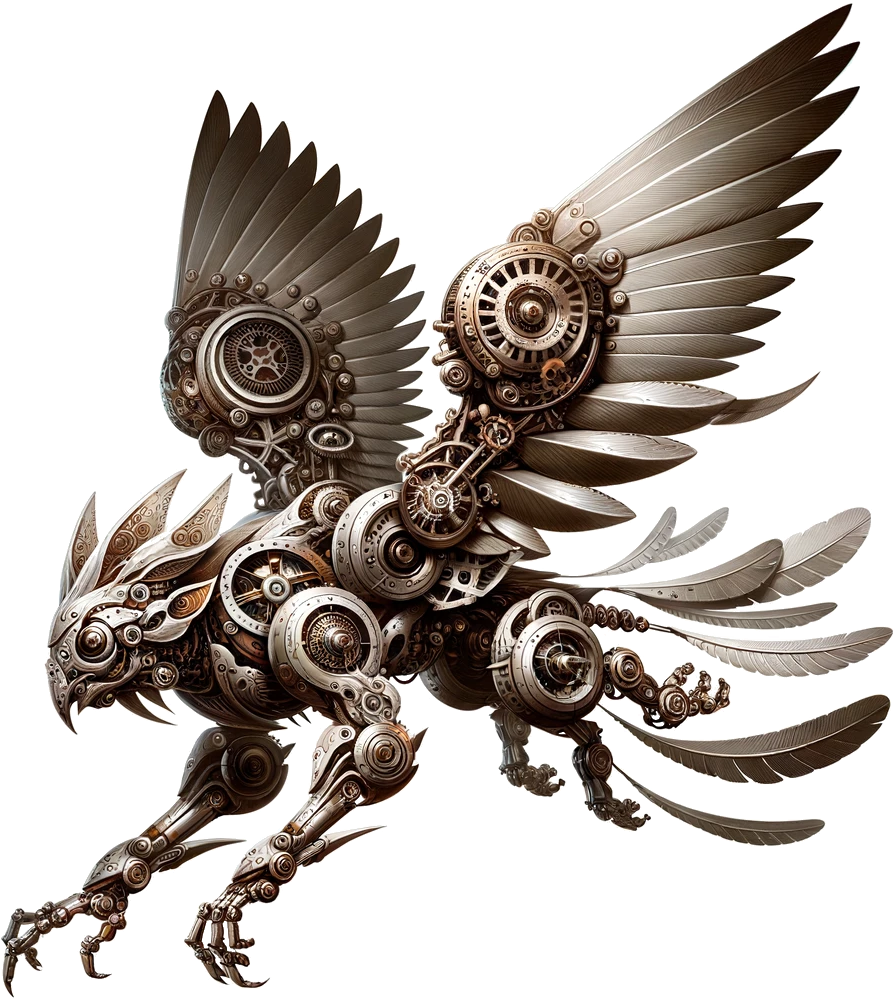
\includegraphics[width=0.175\paperwidth, keepaspectratio]{images/Homunculus_Servant.png}};
\end{tikzpicture}
\noindent\paragraph{Combat} The homunculus is an ally to you and your allies. In combat, it shares your Initiative count, but it takes its turn immediately after yours. It obeys your commands (no action required by you). If you don't issue any, it takes the Dodge action and uses its movement to avoid danger.

\subparagraph*{Using a Higher-Level Spell Slot} Use the spell slot's level for the spell's level in the stat block.
\DndSpellHeader
  {Invisibility}
  {2nd-Level Illusion}
  {Action}
  {Touch}
  {V, S, M (an eyelash in gum arabic)}
  {Concentration, up to 1 Hour}

A creature you touch has the Invisible condition until the spell ends. The spell ends early immediately after the target makes an attack roll, deals damage, or casts a spell.

\subparagraph*{Using a Higher-Level Spell Slot} You can target one additional creature for each spell slot level above 2.
\DndSpellHeader
  {See Invisibility}
  {2nd-Level Divination}
  {Action}
  {Self}
  {V, S, M (a pinch of talc)}
  {1 Hour}

For the duration, you see creatures and objects that have the Invisible condition as if they were visible, and you can see into the Ethereal Plane. Creatures and objects there appear ghostly.
\DndSpellHeader
  {Shining Smite}
  {2nd-Level Transmutation}
  {Bonus Action, which you take immediately after hitting a creature with a Melee weapon or an Unarmed Strike}
  {Self}
  {V}
  {Concentration, up to 1 Minute}

The target hit by the strike takes an extra 2d6 Radiant damage from the attack. Until the spell ends, the target sheds Bright Light in a 5-foot radius, attack rolls against it have Advantage, and it can't benefit from the Invisible condition.

\subparagraph*{Using a Higher-Level Spell Slot} The damage increases by 1d6 for each spell slot level above 2.
\DndSpellHeader
  {Warding Bond}
  {2nd-Level Abjuration}
  {Action}
  {Touch}
  {V, S, M (a pair of platinum rings worth 50+ GP each, which you and the target must wear for the duration)}
  {1 Hour}

You touch another creature that is willing and create a mystic connection between you and the target until the spell ends. While the target is within 60 feet of you, it gains a +1 bonus to AC and saving throws, and it has Resistance to all damage. Also, each time it takes damage, you take the same amount of damage.

The spell ends if you drop to 0 Hit Points or if you and the target become separated by more than 60 feet. It also ends if the spell is cast again on either of the connected creatures.
\clearpage
\section*{Druid Spells}
\subsection*{Cantrip}
\DndSpellHeader
  {Chill Touch}
  {Necromancy Cantrip}
  {Action}
  {Touch}
  {V, S}
  {Instantaneous}

Channeling the chill of the grave, make a melee spell attack against a target within reach. On a hit, the target takes 1d10 Necrotic damage, and it can't regain Hit Points until the end of your next turn.

\subparagraph*{Cantrip Upgrade} The damage increases by 1d10 when you reach levels 5 (2d10), 11 (3d10), and \textbf{17 (4d10)}.
\DndSpellHeader
  {Hunter Sense}
  {Divination Cantrip}
  {Action}
  {Touch}
  {V, S}
  {Concentration, up to 1 Minute}

You touch a willing creature. For the duration, the target's senses are heightened. Whenever the target makes a Wisdom (Perception) check, it can treat a d20 roll of 9 or lower as a 10.
\DndSpellHeader
  {Mysterious Presence}
  {Illusion Cantrip}
  {Action}
  {Touch}
  {V, S}
  {Concentration, up to 1 Minute}

You touch a willing creature and shroud its presence. Until the spell ends, other creatures must subtract 1d4 from any Wisdom (Insight or Perception) checks made against the target.
\DndSpellHeader
  {Spare the Dying}
  {Necromancy Cantrip}
  {Action}
  {120 Feet}
  {V, S}
  {Instantaneous}

Choose a creature within range that has 0 Hit Points and isn't dead. The creature becomes Stable.

\subparagraph*{Cantrip Upgrade} The range doubles when you reach levels 5 (30 feet), 11 (60 feet), and \textbf{17 (120 feet)}.
\DndSpellHeader
  {Thorn Whip}
  {Transmutation Cantrip}
  {Action}
  {30 Feet}
  {V, S, M (the stem of a plant with thorns)}
  {Instantaneous}

You create a vine-like whip covered in thorns that lashes out at your command toward a creature in range. Make a melee spell attack against the target. On a hit, the target takes 1d6 Piercing damage, and if it is Large or smaller, you can pull it up to 10 feet closer to you.

\subparagraph*{Cantrip Upgrade} The damage increases by 1d6 when you reach levels 5 (2d6), 11 (3d6), and \textbf{17 (4d6)}.

\subsection*{Level 1}
\DndSpellHeader
  {Find Familiar}
  {1st-Level Conjuration}
  {1 Hour or Ritual}
  {10 Feet}
  {V, S, M (burning incense worth 10+ GP, which the spell consumes)}
  {Instantaneous}

You gain the service of a familiar, a spirit that takes an animal form you choose: Bat, Cat, Frog, Hawk, Lizard, Octopus, Owl, Rat, Raven, Spider, Weasel, or another Beast that has a Challenge Rating of 0. Appearing in an unoccupied space within range, the familiar has the statistics of the chosen form, though it is a Celestial, Fey, or Fiend (your choice) instead of a Beast. Your familiar acts independently of you, but it obeys your commands.
\paragraph{Telepathic Connection} While your familiar is within 100 feet of you, you can communicate with it telepathically. Additionally, as a Bonus Action, you can see through the familiar's eyes and hear what it hears until the start of your next turn, gaining the benefits of any special senses it has.

Finally, when you cast a spell with a range of touch, your familiar can deliver the touch. Your familiar must be within 100 feet of you, and it must take a Reaction to deliver the touch when you cast the spell.
\paragraph{Combat} The familiar is an ally to you and your allies. It rolls its own Initiative and acts on its own turn. A familiar can't attack, but it can take other actions as normal.
\paragraph{Disappearance of the Familiar} When the familiar drops to 0 Hit Points, it disappears. It reappears after you cast this spell again. As a Magic action, you can temporarily dismiss the familiar to a pocket dimension. Alternatively, you can dismiss it forever. As a Magic action while it is temporarily dismissed, you can cause it to reappear in an unoccupied space within 30 feet of you. Whenever the familiar drops to 0 Hit Points or disappears into the pocket dimension, it leaves behind in its space anything it was wearing or carrying.
\paragraph{One Familiar Only} You can't have more than one familiar at a time. If you cast this spell while you have a familiar, you instead cause it to adopt a new eligible form.
\DndSpellHeader
  {Infect}
  {1st-Level Necromancy}
  {Action}
  {60 Feet}
  {V, S, M (a petri dish)}
  {Concentration, up to 1 Minute}

You inflict a creature you can see within range with a magical disease. At the start of each of the target's turns, it must make a Constitution saving throw. The creature takes 1d12 necrotic damage on a failed saving throw, or half as much on a successful one. If a target succeeds on three of these saves, the spell ends.

A lesser restoration spell cast on the target ends this spell early.

\subparagraph*{Using a Higher-Level Spell Slot} If you cast this spell using a spell slot of 2nd level or higher, the damage increases by 1d12 for every two slot levels above 1st.
\DndSpellHeader
  {Speak with Animals}
  {1st-Level Divination}
  {Action or Ritual}
  {Self}
  {V, S}
  {10 Minutes}

For the duration, you can comprehend and verbally communicate with Beasts, and you can use any of the Influence action's skill options with them.

Most Beasts have little to say about topics that don't pertain to survival or companionship, but at minimum, a Beast can give you information about nearby locations and monsters, including whatever it has perceived within the past day.

\subsection*{Level 2}
\DndSpellHeader
  {Animal Messenger}
  {2nd-Level Enchantment}
  {Action or Ritual}
  {30 Feet}
  {V, S, M (a morsel of food)}
  {24 Hours}

A Tiny Beast of your choice that you can see within range must succeed on a Charisma saving throw, or it attempts to deliver a message for you (if the target's Challenge Rating isn't 0, it automatically succeeds). You specify a location you have visited and a recipient who matches a general description, such as "a person dressed in the uniform of the town guard" or "a red-haired dwarf wearing a pointed hat." You also communicate a message of up to twenty-five words. The Beast travels for the duration toward the specified location, covering about 25 miles per 24 hours or 50 miles if the Beast can fly.

When the Beast arrives, it delivers your message to the creature that you described, mimicking your communication. If the Beast doesn't reach its destination before the spell ends, the message is lost, and the Beast returns to where you cast the spell.

\subparagraph*{Using a Higher-Level Spell Slot} The spell's duration increases by 48 hours for each spell slot level above 2.
\DndSpellHeader
  {Blindness/Deafness}
  {2nd-Level Transmutation}
  {Action}
  {120 Feet}
  {V}
  {1 Minute}

One creature that you can see within range must succeed on a Constitution saving throw, or it has the Blinded or Deafened condition (your choice) for the duration. At the end of each of its turns, the target repeats the save, ending the spell on itself on a success.

\subparagraph*{Using a Higher-Level Spell Slot} You can target one additional creature for each spell slot level above 2.
\DndSpellHeader
  {Gentle Repose}
  {2nd-Level Necromancy}
  {Action or Ritual}
  {Touch}
  {V, S, M (2 Copper Pieces, which the spell consumes)}
  {10 Days}

You touch a corpse or other remains. For the duration, the target is protected from decay and can't become Undead.

The spell also effectively extends the time limit on raising the target from the dead, since days spent under the influence of this spell don't count against the time limit of spells such as Raise Dead.
\DndSpellHeader
  {Heat Metal}
  {2nd-Level Transmutation}
  {Action}
  {60 Feet}
  {V, S, M (a piece of iron and a flame)}
  {Concentration, up to 1 Minute}

Choose a manufactured metal object, such as a metal weapon or a suit of Heavy or Medium metal armor, that you can see within range. You cause the object to glow red-hot. Any creature in physical contact with the object takes 2d8 Fire damage when you cast the spell. Until the spell ends, you can take a Bonus Action on each of your later turns to deal this damage again if the object is within range.

If a creature is holding or wearing the object and takes the damage from it, the creature must succeed on a Constitution saving throw or drop the object if it can. If it doesn't drop the object, it has Disadvantage on attack rolls and ability checks until the start of your next turn.

\subparagraph*{Using a Higher-Level Spell Slot} The damage increases by 1d8 for each spell slot level above 2.
\DndSpellHeader
  {Moonbeam}
  {2nd-Level Evocation}
  {Action}
  {120 Feet}
  {V, S, M (a moonseed leaf)}
  {Concentration, up to 1 Minute}

A silvery beam of pale light shines down in a 5-foot-radius, 40-foot-high Cylinder centered on a point within range. Until the spell ends, Dim Light fills the Cylinder, and you can take a Magic action on later turns to move the Cylinder up to 60 feet.

When the Cylinder appears, each creature in it makes a Constitution saving throw. On a failed save, a creature takes 2d10 Radiant damage, and if the creature is shape-shifted (as a result of the Polymorph spell, for example), it reverts to its true form and can't shape-shift until it leaves the Cylinder. On a successful save, a creature takes half as much damage only. A creature also makes this save when the spell's area moves into its space and when it enters the spell's area or ends its turn there. A creature makes this save only once per turn.

\subsection*{Level 3}
\DndSpellHeader
  {Animate Dead}
  {3rd-Level Necromancy}
  {1 Minute}
  {10 Feet}
  {V, S, M (a drop of blood, a piece of flesh, and a pinch of bone dust)}
  {Instantaneous}

Choose a pile of bones or a corpse of a Medium or Small Humanoid within range. The target becomes an Undead creature: a Skeleton if you chose bones or a Zombie if you chose a corpse.

On each of your turns, you can take a Bonus Action to mentally command any creature you made with this spell if the creature is within 60 feet of you (if you control multiple creatures, you can command any of them at the same time, issuing the same command to each one). You decide what action the creature will take and where it will move on its next turn, or you can issue a general command, such as to guard a chamber or corridor. If you issue no commands, the creature takes the Dodge action and moves only to avoid harm. Once given an order, the creature continues to follow it until its task is complete.

The creature is under your control for 24 hours, after which it stops obeying any command you've given it. To maintain control of the creature for another 24 hours, you must cast this spell on the creature again before the current 24-hour period ends. This use of the spell reasserts your control over up to four creatures you have animated with this spell rather than animating a new creature.

\subparagraph*{Using a Higher-Level Spell Slot} You animate or reassert control over two additional Undead creatures for each spell slot level above 3. Each of the creatures must come from a different corpse or pile of bones.
\DndSpellHeader
  {Dispel Magic}
  {3rd-Level Abjuration}
  {Action}
  {120 Feet}
  {V, S}
  {Instantaneous}

Choose one creature, object, or magical effect within range. Any ongoing spell of level 3 or lower on the target ends. For each ongoing spell of level 4 or higher on the target, make an ability check using your spellcasting ability (DC 10 plus that spell's level). On a successful check, the spell ends.

\subparagraph*{Using a Higher-Level Spell Slot} You automatically end a spell on the target if the spell's level is equal to or less than the level of the spell slot you use.
\DndSpellHeader
  {Elemental Exhalation}
  {3rd-Level Evocation}
  {Action}
  {Self}
  {S}
  {Instantaneous}

When you cast this spell, choose one of the following effects that determine the spell's damage type:
\paragraph{Air} The damage type is Thunder. Each creature that fails the saving throw is pushed 10 feet away from you.
\paragraph{Coldfire} The damage type is Cold. Each creature that fails the saving throw has the Frightened condition until the start of your next turn.
\paragraph{Earth} The damage type is Bludgeoning. Each creature that fails the saving throw has its Speed reduced to 0 until the end of its next turn.
\paragraph{Fire} The damage type is Fire. Each creature that fails the saving throw is engulfed in flames and takes 2d6 Fire damage at the end of its next turn. As an action, it can extinguish fire on itself by giving itself the Prone condition and rolling on the ground. The fire also goes out if it is doused, submerged, or suffocated.
\paragraph{Water} The damage type is Acid. Each creature that fails the saving throw has the Prone condition.

Each creature within a 30-foot Cone of destructive elemental energy must make a Dexterity saving throw. On a failed save, a target takes 5d6 damage of the chosen type. On a successful save, the target takes half as much damage only.

\subparagraph*{Using a Higher-Level Spell Slot} The damage increases by 1d6 for each spell slot level above 3.
\DndSpellHeader
  {Erupting Earth}
  {3rd-Level Transmutation}
  {Action}
  {120 Feet}
  {V, S, M (a piece of obsidian)}
  {Instantaneous}

Choose a point you can see on the ground within range. A fountain of churned earth and stone erupts in a 20-foot cube centered on that point. Each creature in that area must make a Dexterity saving throw. A creature takes 3d12 bludgeoning damage on a failed save, or half as much damage on a successful one. Additionally, the ground in that area becomes difficult terrain until cleared. Each 5-foot-square portion of the area requires at least 1 minute to clear by hand.

\subparagraph*{Using a Higher-Level Spell Slot} When you cast this spell using a spell slot of 4th level or higher, the damage increases by 1d12 for each slot level above 3rd.
\DndSpellHeader
  {Feign Death}
  {3rd-Level Necromancy}
  {Action or Ritual}
  {Touch}
  {V, S, M (a pinch of graveyard dirt)}
  {1 Hour}

You touch a willing creature and put it into a cataleptic state that is indistinguishable from death.

For the duration, the target appears dead to outward inspection and to spells used to determine the target's status. The target has the Blinded and Incapacitated conditions, and its Speed is 0.

The target also has Resistance to all damage except Psychic damage, and it has Immunity to the Poisoned condition.
\DndSpellHeader
  {Gaseous Form}
  {3rd-Level Transmutation}
  {Action}
  {Touch}
  {V, S, M (a bit of gauze)}
  {Concentration, up to 1 Hour}

A willing creature you touch shape-shifts, along with everything it's wearing and carrying, into a misty cloud for the duration. The spell ends on the target if it drops to 0 Hit Points or if it takes a Magic action to end the spell on itself.

While in this form, the target's only method of movement is a Fly Speed of 10 feet, and it can hover. The target can enter and occupy the space of another creature. The target has Resistance to Bludgeoning, Piercing, and Slashing damage; it has Immunity to the Prone condition; and it has Advantage on Strength, Dexterity, and Constitution saving throws. The target can pass through narrow openings, but it treats liquids as though they were solid surfaces.

The target can't talk or manipulate objects, and any objects it was carrying or holding can't be dropped, used, or otherwise interacted with. Finally, the target can't attack or cast spells.

\subparagraph*{Using a Higher-Level Spell Slot} You can target one additional creature for each spell slot level above 3.
\DndSpellHeader
  {Pestilence}
  {3rd-Level Necromancy}
  {Action}
  {90 Feet}
  {V, S, M (a withered flower)}
  {Concentration, up to 1 Minute}

You infect up to three creatures you can see within range with a magical disease. At the start of each of the target's turns, it must make a Constitution saving throw. On a failed saving throw, the creature takes 3d6 necrotic damage and gains 1 level of exhaustion. If a target succeeds on three of these saves, the spell ends for that creature.

\DndSpellHeader
  {Scarlet Dawn}
  {3rd-Level Evocation}
  {Action}
  {120 Feet}
  {V, S}
  {Instantaneous}

Crimson light shines down in a 20-foot-radius, 60-foot-high Cylinder centered on a point within range. Each creature in that area that isn't a Construct or Undead must make a Constitution saving throw, taking 4d10 Necrotic damage on a failed save or half as much damage on a successful one. Constructs and Undead in the area regain 4d10 Hit Points.

If any of this spell's area overlaps with an area of Darkness created by a spell of level 3 or lower, that other spell is dispelled.

\subparagraph*{Using a Higher-Level Spell Slot} The damage increases by 1d10 and the level of spell that can be dispelled increases by 1 for each spell slot level above 3.

A lesser restoration spell cast on a target ends this spell early for that creature.
\clearpage
\section*{Ranger Spells}
\subsection*{Level 1}
\DndSpellHeader
  {Ensnaring Strike}
  {1st-Level Conjuration}
  {Bonus Action, which you take immediately after hitting a creature with a weapon}
  {Self}
  {V}
  {Concentration, up to 1 Minute}
  
As you hit the target, grasping vines appear on it, and it makes a Strength saving throw. A Large or larger creature has Advantage on this save. On a failed save, the target has the Restrained condition until the spell ends. On a successful save, the vines shrivel away, and the spell ends.

While Restrained, the target takes 1d6 Piercing damage at the start of each of its turns. The target or a creature within reach of it can take an action to make a Strength (Athletics) check against your spell save DC. On a success, the spell ends.

\subparagraph*{Using a Higher-Level Spell Slot} The damage increases by 1d6 for each spell slot level above 1.
\DndSpellHeader
  {Hail of Thorns}
  {1st-Level Conjuration}
  {Bonus Action, which you take immediately after hitting a creature with a Ranged weapon}
  {Self}
  {V}
  {Instantaneous}
  
As you hit the creature, this spell creates a rain of thorns that sprouts from your Ranged weapon or ammunition. The target of the attack and each creature within 5 feet of it make a Dexterity saving throw, taking 1d10 Piercing damage on a failed save or half as much damage on a successful one.

\subparagraph*{Using a Higher-Level Spell Slot} The damage increases by 1d10 for each spell slot level above 1.
\DndSpellHeader
  {Hungering Blade}
  {1st-Level Necromancy}
  {Bonus Action}
  {Self}
  {V, S}
  {1 Minute}
  
You imbue a weapon you are holding, or your Unarmed Strikes, with ravenous negative energy. For the duration, when you hit a creature with an attack using the empowered weapon or Unarmed Strike for the first time on a turn, the target takes Necrotic damage equal to your spellcasting ability modifier, and you gain a number of Temporary Hit Points equal to the Necrotic damage dealt.
\DndSpellHeader
  {Hunter's Mark}
  {1st-Level Divination}
  {Bonus Action}
  {90 Feet}
  {V}
  {Concentration, up to 1 Hour}
  
You magically mark one creature you can see within range as your quarry. Until the spell ends, you deal an extra 1d6 Force damage to the target whenever you hit it with an attack roll. You also have Advantage on any Wisdom (Perception or Survival) check you make to find it.

If the target drops to 0 Hit Points before this spell ends, you can take a Bonus Action to move the mark to a new creature you can see within range.

\subparagraph*{Using a Higher-Level Spell Slot} Your Concentration can last longer with a spell slot of level 3-4 (up to 8 hours) or 5+ (up to 24 hours).
\DndSpellHeader
  {Protection from Evil and Good}
  {1st-Level Abjuration}
  {Action}
  {Touch}
  {V, S, M (a flask of Holy Water worth 25+ GP, which the spell consumes)}
  {Concentration, up to 10 Minutes}
  
Until the spell ends, one willing creature you touch is protected against creatures that are Aberrations, Celestials, Elementals, Fey, Fiends, or Undead. The protection grants several benefits. Creatures of those types have Disadvantage on attack rolls against the target. The target also can't be possessed by or gain the Charmed or Frightened conditions from them. If the target is already possessed, Charmed, or Frightened by such a creature, the target has Advantage on any new saving throw against the relevant effect.
\DndSpellHeader
  {Thorn Armor}
  {1st-Level Abjuration}
  {Action}
  {Touch}
  {V, S, M (a rose)}
  {10 Minutes}
  
When you cast this spell, a flexible exoskeleton covered in thorns appears around a willing target within range. The target gains 3d6 Temporary Hit Points. If a creature hits the target with a melee attack roll before the spell ends, that creature takes Piercing damage equal to the number of Temporary Hit Points lost as a result of the attack. This spell ends early if the target has no remaining Temporary Hit Points granted by this spell.

\subparagraph*{Using a Higher-Level Spell Slot} The target gains an additional 2d6 Temporary Hit Points for each spell slot level above 1.
\clearpage
\section*{Bard Spells}
\subsection*{Cantrip}
\DndSpellHeader
  {Illusory Instrument}
  {Illusion Cantrip}
  {Action}
  {Touch}
  {V, S}
  {10 Minutes}

You create an illusionary copy of a mundane musical instrument. The copy of the instrument takes on the shape of your fondest memory of the instrument, such as the first flute you owned or the half harp gifted to you by a loved one. This illusion moves as its physical counterpart would, but it is weightless and is tangible only to you. This instrument can be used as a Spellcasting Focus. This illusory instrument dissipates if you move 10 feet away from it orchoose to end the spell (no action required by you).

As a Bonus Action, you can command your instrument to create one of the following effects:
\begin{itemize}
	\item Mimic basic sounds heard on a daily basis, such as a bird chirping, footsteps, or a slamming door.
	\item Automatically play a basic beat at the tempo of your choice.
	\item Record anything played on it, and play it back on a loop.
	\item Record and playback any noise that it could pick up within 15 feet, such as conversation, a royal decree, or a snoring party member who swears that they don't snore.
\end{itemize}
\DndSpellHeader
  {Vicious Mockery}
  {Enchantment Cantrip}
  {Action}
  {60 Feet}
  {V}
  {Instantaneous}

You unleash a string of insults laced with subtle enchantments at one creature you can see or hear within range. The target must succeed on a Wisdom saving throw or take 1d6 Psychic damage and have Disadvantage on the next attack roll it makes before the end of its next turn.

\subparagraph*{Cantrip Upgrade} The damage increases by 1d6 when you reach levels 5 (2d6), 11 (3d6), and \textbf{17 (4d6)}.

\subsection*{Level 1}
\DndSpellHeader
  {Charm Person}
  {1st-Level Enchantment}
  {Action}
  {30 Feet}
  {V, S}
  {1 Hour}

One Humanoid you can see within range makes a Wisdom saving throw. It does so with Advantage if you or your allies are fighting it. On a failed save, the target has the Charmed condition until the spell ends or until you or your allies damage it. The Charmed creature is Friendly to you. When the spell ends, the target knows it was Charmed by you.

\subparagraph*{Using a Higher-Level Spell Slot} You can target one additional creature for each spell slot level above 1.
\DndSpellHeader
  {Distort Value}
  {1st-Level Illusion}
  {1 Minute}
  {Touch}
  {V}
  {8 Hours}

Do you need to squeeze a few more gold pieces out of a merchant as you try to sell that weird octopus statue you liberated from the chaos temple? Do you need to downplay the worth of some magical assets when the tax collector stops by? Distort value has you covered.

You cast this spell on an object no more than 1 foot on a side, doubling the object's perceived value by adding illusory flourishes or polish to it, or reducing its perceived value by half with the help of illusory scratches, dents, and other unsightly features. Anyone examining the object can ascertain its true value with a successful Intelligence (Investigation) check against your spell save DC.

\subparagraph*{Using a Higher-Level Spell Slot} When you cast this spell using a spell slot of 2nd level or higher, the maximum size of the object increases by 1 foot for each slot level above 1st.
\DndSpellHeader
  {Comprehend Languages}
  {1st-Level Divination}
  {Action or Ritual}
  {Self}
  {V, S, M (a pinch of soot and salt)}
  {1 Hour}

For the duration, you understand the literal meaning of any language that you hear or see signed. You also understand any written language that you see, but you must be touching the surface on which the words are written. It takes about 1 minute to read one page of text. This spell doesn't decode symbols or secret messages.
\DndSpellHeader
  {Illusory Script}
  {1st-Level Illusion}
  {1 Minute or Ritual}
  {Touch}
  {S, M (ink worth 10+ GP, which the spell consumes)}
  {10 Days}

You write on parchment, paper, or another suitable material and imbue it with an illusion that lasts for the duration. To you and any creatures you designate when you cast the spell, the writing appears normal, seems to be written in your hand, and conveys whatever meaning you intended when you wrote the text. To all others, the writing appears as if it were written in an unknown or magical script that is unintelligible. Alternatively, the illusion can alter the meaning, handwriting, and language of the text, though the language must be one you know.

If the spell is dispelled, the original script and the illusion both disappear.

A creature that has Truesight can read the hidden message.
\DndSpellHeader
  {Unseen Servant}
  {1st-Level Conjuration}
  {Action or Ritual}
  {60 Feet}
  {V, S, M (a bit of string and of wood)}
  {1 Hour}

This spell creates an Invisible, mindless, shapeless, Medium force that performs simple tasks at your command until the spell ends. The servant springs into existence in an unoccupied space on the ground within range. It has AC 10, 1 Hit Point, and a Strength of 2, and it can't attack. If it drops to 0 Hit Points, the spell ends.

Once on each of your turns as a Bonus Action, you can mentally command the servant to move up to 15 feet and interact with an object. The servant can perform simple tasks that a human could do, such as fetching things, cleaning, mending, folding clothes, lighting fires, serving food, and pouring drinks. Once you give the command, the servant performs the task to the best of its ability until it completes the task, then waits for your next command.

If you command the servant to perform a task that would move it more than 60 feet away from you, the spell ends.
\clearpage
\section*{Sorcerer Spells}
\subsection*{Cantrip}
\DndSpellHeader
  {Elementalism}
  {Transmutation Cantrip}
  {Action}
  {30 Feet}
  {V, S}
  {Instantaneous}
  
You exert control over the elements, creating one of the following effects within range.
\paragraph{Beckon Air} You create a breeze strong enough to ripple cloth, stir dust, rustle leaves, and close open doors and shutters, all in a 5-foot Cube. Doors and shutters being held open by someone or something aren't affected.
\paragraph{Beckon Earth} You create a thin shroud of dust or sand that covers surfaces in a 5-foot-square area, or you cause a single word to appear in your handwriting in a patch of dirt or sand.
\paragraph{Beckon Fire} You create a thin cloud of harmless embers and colored, scented smoke in a 5-foot Cube. You choose the color and scent, and the embers can light candles, torches, or lamps in that area. The smoke's scent lingers for 1 minute.
\paragraph{Beckon Water} You create a spray of cool mist that lightly dampens creatures and objects in a 5-foot Cube. Alternatively, you create 1 cup of clean water either in an open container or on a surface, and the water evaporates in 1 minute.
\paragraph{Sculpt Element} You cause dirt, sand, fire, smoke, mist, or water that can fit in a 1-foot Cube to assume a crude shape (such as that of a creature) for 1 hour.
\DndSpellHeader
  {Mage Hand}
  {Conjuration Cantrip}
  {Action}
  {30 Feet}
  {V, S}
  {1 Minute}

A spectral, floating hand appears at a point you choose within range. The hand lasts for the duration. The hand vanishes if it is ever more than 30 feet away from you or if you cast this spell again.

When you cast the spell, you can use the hand to manipulate an object, open an unlocked door or container, stow or retrieve an item from an open container, or pour the contents out of a vial.

As a Magic action on your later turns, you can control the hand thus again. As part of that action, you can move the hand up to 30 feet.

The hand can't attack, activate magic items, or carry more than 10 pounds.
\DndSpellHeader
  {Shocking Grasp}
  {Evocation Cantrip}
  {Action}
  {Touch}
  {V, S}
  {Instantaneous}

Lightning springs from you to a creature that you try to touch. Make a melee spell attack against the target. On a hit, the target takes 1d8 Lightning damage, and it can't make Opportunity Attacks until the start of its next turn.

\subparagraph*{Cantrip Upgrade} The damage increases by 1d8 when you reach levels 5 (2d8), 11 (3d8), and \textbf{17 (4d8)}.
\DndSpellHeader
  {Sorcerous Burst}
  {Evocation Cantrip}
  {Action}
  {120 Feet}
  {V, S}
  {Instantaneous}

You cast sorcerous energy at one creature or object within range. Make a ranged attack roll against the target. On a hit, the target takes 1d8 damage of a type you choose: Acid, Cold, Fire, Lightning, Poison, Psychic, or Thunder.

If you roll an 8 on a d8 for this spell, you can roll another d8, and add it to the damage. When you cast this spell, the maximum number of these d8s you can add to the spell's damage equals your spellcasting ability modifier.

\subparagraph*{Cantrip Upgrade} The damage increases by 1d8 when you reach levels 5 (2d8), 11 (3d8), and \textbf{17 (4d8}).

\subsection*{Level 1}
\DndSpellHeader
  {Chromatic Orb}
  {1st-Level Evocation}
  {Action}
  {90 Feet}
  {V, S, M (a diamond worth 50+ GP)}
  {Instantaneous}

You hurl an orb of energy at a target within range. Choose Acid, Cold, Fire, Lightning, Poison, or Thunder for the type of orb you create, and then make a ranged spell attack against the target. On a hit, the target takes 3d8 damage of the chosen type.

If you roll the same number on two or more of the d8s, the orb leaps to a different target of your choice within 30 feet of the target. Make an attack roll against the new target, and make a new damage roll. The orb can't leap again unless you cast the spell with a level 2+ spell slot.

\subparagraph*{Using a Higher-Level Spell Slot} The damage increases by 1d8 for each spell slot level above 1. The orb can leap a maximum number of times equal to the level of the slot expended, and a creature can be targeted only once by each casting of this spell.
\DndSpellHeader
  {Witch Bolt}
  {1st-Level Evocation}
  {Action}
  {60 Feet}
  {V, S, M (a twig struck by lightning)}
  {Concentration, up to 1minute}

A beam of crackling energy lances toward a creature within range, forming a sustained arc of lightning between you and the target. Make a ranged spell attack against it. On a hit, the target takes 2d12 Lightning damage.

On each of your subsequent turns, you can take a Bonus Action to deal 1d12 Lightning damage to the target automatically, even if the first attack missed.

The spell ends if the target is ever outside the spell's range or if it has Total Cover from you.

\subparagraph*{Using a Higher-Level Spell Slot} The initial damage increases by 1d12 for each spell slot level above 1.
\clearpage
\section*{Miscellaneous}
\subsection*{Attack and Damage Rolls}
\subsubsection*{Melee Weapons}
\paragraph*{Attack Roll}\hfill\\
\underline{\textit{Mace:}}\\
1d20 + STR-Modifier + Proficiency Modifier\\
\indent Current Max: \intcalcAdd{20}{\intcalcAdd{\calculateModifier{\StrengthScoreValue}}{\ProficiencyValue}}
\\
\underline{\textit{Rapier (Finesse):}}\\
1d20 + DEX-Modifier + Proficiency Modifier\\
\indent Current Max: \intcalcAdd{20}{\intcalcAdd{\calculateModifier{\DexterityScoreValue}}{\ProficiencyValue}}
\\
\underline{\textit{Handaxe (Throwable):}}\\
1d20 + STR-Modifier + Proficiency Modifier\\
\indent Current Max (melee): \intcalcAdd{20}{\intcalcAdd{\calculateModifier{\StrengthScoreValue}}{\ProficiencyValue}}\\
\indent Current Max (thrown): \intcalcAdd{20}{\intcalcAdd{\calculateModifier{\StrengthScoreValue}}{\ProficiencyValue}}
\\
\underline{\textit{Quarterstaff (Versatile):}}\\
1d20 + STR-Modifier + Proficiency Modifier\\
\indent Current Max: \intcalcAdd{20}{\intcalcAdd{\calculateModifier{\StrengthScoreValue}}{\ProficiencyValue}}
\paragraph*{Damage Roll}\hfill\\
\underline{\textit{Mace:}}\\
1d6 + STR-Modifier\\
\indent Current Max: \intcalcAdd{6}{\calculateModifier{\StrengthScoreValue}}
\\
\underline{\textit{Rapier (Finesse):}}\\
1d8 + DEX-Modifier\\
\indent Current Max: \intcalcAdd{8}{\calculateModifier{\DexterityScoreValue}}
\\
\underline{\textit{Handaxe (Throwable):}}\\
1d6 + STR-Modifier\\
\indent Current Max (melee): \intcalcAdd{6}{\calculateModifier{\StrengthScoreValue}}\\
\indent Current Max (thrown): \intcalcAdd{6}{\calculateModifier{\StrengthScoreValue}}
\\
\underline{\textit{Quarterstaff (Versatile):}}\\
1d6 (1d8) + STR-Modifier\\
\indent Current Max (one-handed): \intcalcAdd{6}{\calculateModifier{\StrengthScoreValue}}\\
\indent Current Max (two-handed): \intcalcAdd{8}{\calculateModifier{\StrengthScoreValue}}
\subsubsection*{Ranged Weapons}
\paragraph*{Attack Roll}\hfill\\
\underline{\textit{Shortbow:}}\\
1d20 + DEX-Modifier + Proficiency Modifier\\
\indent Current Max: \intcalcAdd{20}{\intcalcAdd{\calculateModifier{\DexterityScoreValue}}{\ProficiencyValue}}
\paragraph*{Damage Roll}\hfill\\
\underline{\textit{Shortbow:}}\\
1d6 + DEX-Modifier\\
\indent Current Max: \intcalcAdd{6}{\calculateModifier{\DexterityScoreValue}}
\subsubsection*{Special Attacks}
\paragraph*{Attack Roll}\hfill\\
\underline{\textit{Unarmed Strike:}}\\
1d20 + STR-Modifier + Proficiency Modifier\\
\indent Current Max: \intcalcAdd{20}{\intcalcAdd{\calculateModifier{\StrengthScoreValue}}{\ProficiencyValue}}
\paragraph*{Damage Roll}\hfill\\
\underline{\textit{Unarmed Strike:}}\\
1 + STR-Modifier\\
\indent Current Max: \intcalcMax{1}{\intcalcAdd{1}{\calculateModifier{\StrengthScoreValue}}}

\part*{Magic Items}

\subsection*{All-Purpose Tool +3}
\textit{Wondrous Item, Spellcasting Focus, Very Rare (Requires Attunement by an Artificer)}\\
This simple screwdriver can transform into a variety of tools; as an action, you can touch the item and transform it into any type of artisan's tool of your choice (see the "Equipment" chapter in the Player's Handbook for a list of artisan's tools). Whatever form the tool takes, you are proficient with it.

While holding this tool, you gain a +3 bonus to the spell attack rolls and the saving throw DCs of your artificer spells.

As an action, you can focus on the tool to channel your creative forces. Choose a cantrip that you don't know from any class list. For 8 hours, you can cast that cantrip, and it counts as an artificer cantrip for you. Once this property is used, it can't be used again until the next dawn.

\subsection*{Chronolometer}
\textit{Wondrous Item, Very Rare (Requires Attunement)}\\
While attuned to this device, you have a +1 bonus to Intelligence saving throws. The first time you attune to the chronolometer, you choose one language you don't know. You subsequently know that language while attuned to the device.

\paragraph*{Time Bandit} At the start of your turn, roll a d6 (no action required). On a 1-3, you slow down time, gaining an additional action on your turn and doubling your speed until the end of the turn. On a 4-6, you go forward in time to warn yourself of what is to come. The next time you fail a saving throw, attack roll, or ability check, you can reroll the check and take either result. Once you use this feature of the chronolometer, it cannot be used again until the next dawn.

\paragraph*{Fate Swap} As a reaction when a creature you can see within 30 feet of you takes damage, that creature gains an additional action if it is the creature's turn, or can take an action immediately even though it isn't the creature's turn. Once you use this feature of the chronolometer, it cannot be used again until the next dawn.

\paragraph*{Part of a Whole} While this component is not installed in the Orrery of the Wanderer, its magic might function sporadically or with unpredictable side effects, as determined by the DM.

\end{document}